\documentclass[twoside]{book}

% Packages required by doxygen
\usepackage{fixltx2e}
\usepackage{calc}
\usepackage{doxygen}
\usepackage[export]{adjustbox} % also loads graphicx
\usepackage{graphicx}
\usepackage[utf8]{inputenc}
\usepackage{makeidx}
\usepackage{multicol}
\usepackage{multirow}
\PassOptionsToPackage{warn}{textcomp}
\usepackage{textcomp}
\usepackage[nointegrals]{wasysym}
\usepackage[table]{xcolor}

% NLS support packages
\usepackage[french]{babel}

% Font selection
\usepackage[T1]{fontenc}
\usepackage[scaled=.90]{helvet}
\usepackage{courier}
\usepackage{amssymb}
\usepackage{sectsty}
\renewcommand{\familydefault}{\sfdefault}
\allsectionsfont{%
  \fontseries{bc}\selectfont%
  \color{darkgray}%
}
\renewcommand{\DoxyLabelFont}{%
  \fontseries{bc}\selectfont%
  \color{darkgray}%
}
\newcommand{\+}{\discretionary{\mbox{\scriptsize$\hookleftarrow$}}{}{}}

% Page & text layout
\usepackage{geometry}
\geometry{%
  a4paper,%
  top=2.5cm,%
  bottom=2.5cm,%
  left=2.5cm,%
  right=2.5cm%
}
\tolerance=750
\hfuzz=15pt
\hbadness=750
\setlength{\emergencystretch}{15pt}
\setlength{\parindent}{0cm}
\setlength{\parskip}{3ex plus 2ex minus 2ex}
\makeatletter
\renewcommand{\paragraph}{%
  \@startsection{paragraph}{4}{0ex}{-1.0ex}{1.0ex}{%
    \normalfont\normalsize\bfseries\SS@parafont%
  }%
}
\renewcommand{\subparagraph}{%
  \@startsection{subparagraph}{5}{0ex}{-1.0ex}{1.0ex}{%
    \normalfont\normalsize\bfseries\SS@subparafont%
  }%
}
\makeatother

% Headers & footers
\usepackage{fancyhdr}
\pagestyle{fancyplain}
\fancyhead[LE]{\fancyplain{}{\bfseries\thepage}}
\fancyhead[CE]{\fancyplain{}{}}
\fancyhead[RE]{\fancyplain{}{\bfseries\leftmark}}
\fancyhead[LO]{\fancyplain{}{\bfseries\rightmark}}
\fancyhead[CO]{\fancyplain{}{}}
\fancyhead[RO]{\fancyplain{}{\bfseries\thepage}}
\fancyfoot[LE]{\fancyplain{}{}}
\fancyfoot[CE]{\fancyplain{}{}}
\fancyfoot[RE]{\fancyplain{}{\bfseries\scriptsize Généré par Doxygen }}
\fancyfoot[LO]{\fancyplain{}{\bfseries\scriptsize Généré par Doxygen }}
\fancyfoot[CO]{\fancyplain{}{}}
\fancyfoot[RO]{\fancyplain{}{}}
\renewcommand{\footrulewidth}{0.4pt}
\renewcommand{\chaptermark}[1]{%
  \markboth{#1}{}%
}
\renewcommand{\sectionmark}[1]{%
  \markright{\thesection\ #1}%
}

% Indices & bibliography
\usepackage{natbib}
\usepackage[titles]{tocloft}
\setcounter{tocdepth}{3}
\setcounter{secnumdepth}{5}
\makeindex

% Hyperlinks (required, but should be loaded last)
\usepackage{ifpdf}
\ifpdf
  \usepackage[pdftex,pagebackref=true]{hyperref}
\else
  \usepackage[ps2pdf,pagebackref=true]{hyperref}
\fi
\hypersetup{%
  colorlinks=true,%
  linkcolor=blue,%
  citecolor=blue,%
  unicode%
}

% Custom commands
\newcommand{\clearemptydoublepage}{%
  \newpage{\pagestyle{empty}\cleardoublepage}%
}

\usepackage{caption}
\captionsetup{labelsep=space,justification=centering,font={bf},singlelinecheck=off,skip=4pt,position=top}

%===== C O N T E N T S =====

\begin{document}

% Titlepage & ToC
\hypersetup{pageanchor=false,
             bookmarksnumbered=true,
             pdfencoding=unicode
            }
\pagenumbering{roman}
\begin{titlepage}
\vspace*{7cm}
\begin{center}%
{\Large Blokus\+\_\+terminal }\\
\vspace*{1cm}
{\large Généré par Doxygen 1.8.11}\\
\end{center}
\end{titlepage}
\clearemptydoublepage
\tableofcontents
\clearemptydoublepage
\pagenumbering{arabic}
\hypersetup{pageanchor=true}

%--- Begin generated contents ---
\chapter{Index des classes}
\section{Data Structures}
Here are the data structures with brief descriptions\+:\begin{DoxyCompactList}
\item\contentsline{section}{\mbox{\hyperlink{structt__case}{t\+\_\+case}} \\*Définition d\textquotesingle{}une case pour un plateau de Blokus }{\pageref{structt__case}}{}
\item\contentsline{section}{\mbox{\hyperlink{structt__coordonnee}{t\+\_\+coordonnee}} \\*Contient des coordonnées pour une matrice à deux dimensions }{\pageref{structt__coordonnee}}{}
\item\contentsline{section}{\mbox{\hyperlink{structt__liste}{t\+\_\+liste}} }{\pageref{structt__liste}}{}
\item\contentsline{section}{\mbox{\hyperlink{structt__matrice}{t\+\_\+matrice}} }{\pageref{structt__matrice}}{}
\item\contentsline{section}{\mbox{\hyperlink{structt__retour}{t\+\_\+retour}} }{\pageref{structt__retour}}{}
\end{DoxyCompactList}

\chapter{Index des fichiers}
\section{Liste des fichiers}
Liste de tous les fichiers documentés avec une brève description \+:\begin{DoxyCompactList}
\item\contentsline{section}{src/\hyperlink{afficher_8c}{afficher.\+c} \\*Ensemble de fonctions d\textquotesingle{}affichage }{\pageref{afficher_8c}}{}
\item\contentsline{section}{src/{\bfseries afficher.\+h} }{\pageref{afficher_8h}}{}
\item\contentsline{section}{src/\hyperlink{ajouter__piece_8c}{ajouter\+\_\+piece.\+c} \\*Fonctions qui vérifient le placement d\textquotesingle{}une pièce et la placent }{\pageref{ajouter__piece_8c}}{}
\item\contentsline{section}{src/{\bfseries ajouter\+\_\+piece.\+h} }{\pageref{ajouter__piece_8h}}{}
\item\contentsline{section}{src/{\bfseries couleurs.\+h} }{\pageref{couleurs_8h}}{}
\item\contentsline{section}{src/{\bfseries I\+A.\+h} }{\pageref{IA_8h}}{}
\item\contentsline{section}{src/\hyperlink{init__plateau_8c}{init\+\_\+plateau.\+c} \\*Module de fonctions pour le plateau }{\pageref{init__plateau_8c}}{}
\item\contentsline{section}{src/{\bfseries init\+\_\+plateau.\+h} }{\pageref{init__plateau_8h}}{}
\item\contentsline{section}{src/\hyperlink{liste_8c}{liste.\+c} \\*Ensemble de fonctions servants � l\textquotesingle{}utilisation des listes }{\pageref{liste_8c}}{}
\item\contentsline{section}{src/{\bfseries liste.\+h} }{\pageref{liste_8h}}{}
\item\contentsline{section}{src/{\bfseries matrice.\+h} }{\pageref{matrice_8h}}{}
\item\contentsline{section}{src/\hyperlink{menu__pause_8c}{menu\+\_\+pause.\+c} \\*Fonctions de sauvegarde, de chargement et du menu de pause }{\pageref{menu__pause_8c}}{}
\item\contentsline{section}{src/{\bfseries menu\+\_\+pause.\+h} }{\pageref{menu__pause_8h}}{}
\item\contentsline{section}{src/\hyperlink{Partie_8c}{Partie.\+c} \\*Ensemble de fonctions qui font tourner une partie de jeu. Fichier principal }{\pageref{Partie_8c}}{}
\item\contentsline{section}{src/{\bfseries Partie.\+h} }{\pageref{Partie_8h}}{}
\item\contentsline{section}{src/\hyperlink{possibilite_8c}{possibilite.\+c} \\*Ensemble de fonctions relatives aux possibilitees du positionnement d\textquotesingle{}une ou de plusieurs piece avec un plateau donne }{\pageref{possibilite_8c}}{}
\item\contentsline{section}{src/{\bfseries possibilite.\+h} }{\pageref{possibilite_8h}}{}
\item\contentsline{section}{src/\hyperlink{reseau_8c}{reseau.\+c} \\*Module qui permet une connexion T\+CP entre plusieurs ordinateurs }{\pageref{reseau_8c}}{}
\item\contentsline{section}{src/{\bfseries reseau.\+h} }{\pageref{reseau_8h}}{}
\item\contentsline{section}{src/\hyperlink{structures_8h}{structures.\+h} \\*Contient les structures communes du programme }{\pageref{structures_8h}}{}
\item\contentsline{section}{src/\hyperlink{unicode_8c}{unicode.\+c} \\*Fonctions d\textquotesingle{}affichage des cases du plateau avec des caractères unicode }{\pageref{unicode_8c}}{}
\item\contentsline{section}{src/{\bfseries unicode.\+h} }{\pageref{unicode_8h}}{}
\end{DoxyCompactList}

\chapter{Documentation des classes}
\hypertarget{structt__case}{}\section{Référence de la structure t\+\_\+case}
\label{structt__case}\index{t\+\_\+case@{t\+\_\+case}}


Définition d\textquotesingle{}une case pour un plateau de Blokus.  




{\ttfamily \#include $<$structures.\+h$>$}

\subsection*{Attributs publics}
\begin{DoxyCompactItemize}
\item 
\hyperlink{structures_8h_aa9f0f93fc533400ebe242cbb9986ef07}{t\+\_\+couleur} \hyperlink{structt__case_ae871a70afefeefaeb0003ed141d9d06b}{couleur}
\item 
int \hyperlink{structt__case_abfbade6a8fc1927fbdb8dca9c810b1c4}{possible\+\_\+r}
\item 
int \hyperlink{structt__case_aea7d8d23a697e3cd7b07a44e88f5781b}{possible\+\_\+b}
\item 
int \hyperlink{structt__case_a74e4a7aa37b5071dfc9a4da15d88cc7d}{possible\+\_\+v}
\item 
int \hyperlink{structt__case_a7ba4c0e092015a53344116cc2e54f2dc}{possible\+\_\+j}
\end{DoxyCompactItemize}


\subsection{Description détaillée}
Définition d\textquotesingle{}une case pour un plateau de Blokus. 

Elle contient une couleur pour déterminer si la case est occupée ainsi que des booléens pour savoir si la case est utilisable pour un joueur 

\subsection{Documentation des données membres}
\index{t\+\_\+case@{t\+\_\+case}!couleur@{couleur}}
\index{couleur@{couleur}!t\+\_\+case@{t\+\_\+case}}
\subsubsection[{\texorpdfstring{couleur}{couleur}}]{\setlength{\rightskip}{0pt plus 5cm}{\bf t\+\_\+couleur} t\+\_\+case\+::couleur}\hypertarget{structt__case_ae871a70afefeefaeb0003ed141d9d06b}{}\label{structt__case_ae871a70afefeefaeb0003ed141d9d06b}
énumération qui indique si la case est occupée et par quelle couleur \index{t\+\_\+case@{t\+\_\+case}!possible\+\_\+b@{possible\+\_\+b}}
\index{possible\+\_\+b@{possible\+\_\+b}!t\+\_\+case@{t\+\_\+case}}
\subsubsection[{\texorpdfstring{possible\+\_\+b}{possible_b}}]{\setlength{\rightskip}{0pt plus 5cm}int t\+\_\+case\+::possible\+\_\+b}\hypertarget{structt__case_aea7d8d23a697e3cd7b07a44e88f5781b}{}\label{structt__case_aea7d8d23a697e3cd7b07a44e88f5781b}
booléen qui est vrai si la case est une possibilité pour le joueur bleu \index{t\+\_\+case@{t\+\_\+case}!possible\+\_\+j@{possible\+\_\+j}}
\index{possible\+\_\+j@{possible\+\_\+j}!t\+\_\+case@{t\+\_\+case}}
\subsubsection[{\texorpdfstring{possible\+\_\+j}{possible_j}}]{\setlength{\rightskip}{0pt plus 5cm}int t\+\_\+case\+::possible\+\_\+j}\hypertarget{structt__case_a7ba4c0e092015a53344116cc2e54f2dc}{}\label{structt__case_a7ba4c0e092015a53344116cc2e54f2dc}
booléen qui est vrai si la case est une possibilité pour le joueur jaune \index{t\+\_\+case@{t\+\_\+case}!possible\+\_\+r@{possible\+\_\+r}}
\index{possible\+\_\+r@{possible\+\_\+r}!t\+\_\+case@{t\+\_\+case}}
\subsubsection[{\texorpdfstring{possible\+\_\+r}{possible_r}}]{\setlength{\rightskip}{0pt plus 5cm}int t\+\_\+case\+::possible\+\_\+r}\hypertarget{structt__case_abfbade6a8fc1927fbdb8dca9c810b1c4}{}\label{structt__case_abfbade6a8fc1927fbdb8dca9c810b1c4}
booléen qui est vrai si la case est une possibilité pour le joueur rouge \index{t\+\_\+case@{t\+\_\+case}!possible\+\_\+v@{possible\+\_\+v}}
\index{possible\+\_\+v@{possible\+\_\+v}!t\+\_\+case@{t\+\_\+case}}
\subsubsection[{\texorpdfstring{possible\+\_\+v}{possible_v}}]{\setlength{\rightskip}{0pt plus 5cm}int t\+\_\+case\+::possible\+\_\+v}\hypertarget{structt__case_a74e4a7aa37b5071dfc9a4da15d88cc7d}{}\label{structt__case_a74e4a7aa37b5071dfc9a4da15d88cc7d}
booléen qui est vrai si la case est une possibilité pour le joueur vert 

La documentation de cette structure a été générée à partir du fichier suivant \+:\begin{DoxyCompactItemize}
\item 
src/\hyperlink{structures_8h}{structures.\+h}\end{DoxyCompactItemize}

\hypertarget{structt__coordonnee}{}\section{t\+\_\+coordonnee Struct Reference}
\label{structt__coordonnee}\index{t\+\_\+coordonnee@{t\+\_\+coordonnee}}


Contient des coordonnées pour une matrice à deux dimensions.  




{\ttfamily \#include $<$structures.\+h$>$}

\subsection*{Data Fields}
\begin{DoxyCompactItemize}
\item 
int \mbox{\hyperlink{structt__coordonnee_a6150e0515f7202e2fb518f7206ed97dc}{x}}
\item 
int \mbox{\hyperlink{structt__coordonnee_a0a2f84ed7838f07779ae24c5a9086d33}{y}}
\end{DoxyCompactItemize}


\subsection{Detailed Description}
Contient des coordonnées pour une matrice à deux dimensions. 

\subsection{Field Documentation}
\mbox{\Hypertarget{structt__coordonnee_a6150e0515f7202e2fb518f7206ed97dc}\label{structt__coordonnee_a6150e0515f7202e2fb518f7206ed97dc}} 
\index{t\+\_\+coordonnee@{t\+\_\+coordonnee}!x@{x}}
\index{x@{x}!t\+\_\+coordonnee@{t\+\_\+coordonnee}}
\subsubsection{\texorpdfstring{x}{x}}
{\footnotesize\ttfamily int x}

Numéro de colonne \mbox{\Hypertarget{structt__coordonnee_a0a2f84ed7838f07779ae24c5a9086d33}\label{structt__coordonnee_a0a2f84ed7838f07779ae24c5a9086d33}} 
\index{t\+\_\+coordonnee@{t\+\_\+coordonnee}!y@{y}}
\index{y@{y}!t\+\_\+coordonnee@{t\+\_\+coordonnee}}
\subsubsection{\texorpdfstring{y}{y}}
{\footnotesize\ttfamily int y}

Numéro de ligne 

The documentation for this struct was generated from the following file\+:\begin{DoxyCompactItemize}
\item 
\mbox{\hyperlink{structures_8h}{structures.\+h}}\end{DoxyCompactItemize}

\hypertarget{structt__liste}{}\section{t\+\_\+liste Struct Reference}
\label{structt__liste}\index{t\+\_\+liste@{t\+\_\+liste}}
\subsection*{Data Fields}
\begin{DoxyCompactItemize}
\item 
\mbox{\Hypertarget{structt__liste_a404442353660d7effc914ba8220ebf7f}\label{structt__liste_a404442353660d7effc914ba8220ebf7f}} 
int {\bfseries queue}
\item 
\mbox{\Hypertarget{structt__liste_a59e5dec85b6fd6e9ce7498410e234982}\label{structt__liste_a59e5dec85b6fd6e9ce7498410e234982}} 
int {\bfseries ec}
\item 
\mbox{\Hypertarget{structt__liste_a3cad0928b3a2acd391b940070b2080f0}\label{structt__liste_a3cad0928b3a2acd391b940070b2080f0}} 
\mbox{\hyperlink{structt__matrice}{t\+\_\+matrice}} {\bfseries elem} \mbox{[}T\+A\+I\+L\+L\+E\+\_\+\+M\+AX\mbox{]}
\end{DoxyCompactItemize}


The documentation for this struct was generated from the following file\+:\begin{DoxyCompactItemize}
\item 
liste.\+h\end{DoxyCompactItemize}

\hypertarget{structt__matrice}{}\section{Référence de la structure t\+\_\+matrice}
\label{structt__matrice}\index{t\+\_\+matrice@{t\+\_\+matrice}}
\subsection*{Attributs publics}
\begin{DoxyCompactItemize}
\item 
int {\bfseries mat} \mbox{[}5\mbox{]}\mbox{[}5\mbox{]}\hypertarget{structt__matrice_a0fbccd86aa607efff74de103029b3da0}{}\label{structt__matrice_a0fbccd86aa607efff74de103029b3da0}

\item 
int {\bfseries taille}\hypertarget{structt__matrice_a4df902007b2c86629d7f117a662d4485}{}\label{structt__matrice_a4df902007b2c86629d7f117a662d4485}

\item 
int {\bfseries num}\hypertarget{structt__matrice_ac7b3db002a24749884aeac8bc1a05ab1}{}\label{structt__matrice_ac7b3db002a24749884aeac8bc1a05ab1}

\end{DoxyCompactItemize}


La documentation de cette structure a été générée à partir du fichier suivant \+:\begin{DoxyCompactItemize}
\item 
src/matrice.\+h\end{DoxyCompactItemize}

\hypertarget{structt__retour}{}\section{t\+\_\+retour Struct Reference}
\label{structt__retour}\index{t\+\_\+retour@{t\+\_\+retour}}
\subsection*{Data Fields}
\begin{DoxyCompactItemize}
\item 
int \mbox{\hyperlink{structt__retour_a6623c6e672e749d7cfdf08830bbc5a13}{nb\+\_\+rota}}
\item 
int \mbox{\hyperlink{structt__retour_a48696256120eb2569549fbf206502ce1}{numero\+\_\+piece}}
\item 
int \mbox{\hyperlink{structt__retour_a8afc85cb27005e2bd7dfc73222b85a46}{resultat}}
\item 
\mbox{\hyperlink{structt__coordonnee}{t\+\_\+coordonnee}} \mbox{\hyperlink{structt__retour_a41604ec3aac6c0abd76056239bf73f28}{coord}}
\end{DoxyCompactItemize}


\subsection{Field Documentation}
\mbox{\Hypertarget{structt__retour_a41604ec3aac6c0abd76056239bf73f28}\label{structt__retour_a41604ec3aac6c0abd76056239bf73f28}} 
\index{t\+\_\+retour@{t\+\_\+retour}!coord@{coord}}
\index{coord@{coord}!t\+\_\+retour@{t\+\_\+retour}}
\subsubsection{\texorpdfstring{coord}{coord}}
{\footnotesize\ttfamily \mbox{\hyperlink{structt__coordonnee}{t\+\_\+coordonnee}} coord}

Coordonnee ou il faut placer la piece \mbox{\Hypertarget{structt__retour_a6623c6e672e749d7cfdf08830bbc5a13}\label{structt__retour_a6623c6e672e749d7cfdf08830bbc5a13}} 
\index{t\+\_\+retour@{t\+\_\+retour}!nb\+\_\+rota@{nb\+\_\+rota}}
\index{nb\+\_\+rota@{nb\+\_\+rota}!t\+\_\+retour@{t\+\_\+retour}}
\subsubsection{\texorpdfstring{nb\+\_\+rota}{nb\_rota}}
{\footnotesize\ttfamily int nb\+\_\+rota}

Nombre de rotation a effectuer \mbox{\Hypertarget{structt__retour_a48696256120eb2569549fbf206502ce1}\label{structt__retour_a48696256120eb2569549fbf206502ce1}} 
\index{t\+\_\+retour@{t\+\_\+retour}!numero\+\_\+piece@{numero\+\_\+piece}}
\index{numero\+\_\+piece@{numero\+\_\+piece}!t\+\_\+retour@{t\+\_\+retour}}
\subsubsection{\texorpdfstring{numero\+\_\+piece}{numero\_piece}}
{\footnotesize\ttfamily int numero\+\_\+piece}

Numeros de la piece a retrouver \mbox{\Hypertarget{structt__retour_a8afc85cb27005e2bd7dfc73222b85a46}\label{structt__retour_a8afc85cb27005e2bd7dfc73222b85a46}} 
\index{t\+\_\+retour@{t\+\_\+retour}!resultat@{resultat}}
\index{resultat@{resultat}!t\+\_\+retour@{t\+\_\+retour}}
\subsubsection{\texorpdfstring{resultat}{resultat}}
{\footnotesize\ttfamily int resultat}

Definie le nombre de point que nous offre la piece 

The documentation for this struct was generated from the following file\+:\begin{DoxyCompactItemize}
\item 
I\+A.\+h\end{DoxyCompactItemize}

\chapter{Documentation des fichiers}
\hypertarget{afficher_8c}{}\section{Référence du fichier /info/etu/l2info/l2info031/\+Projet\+\_\+blokus-\/\+Version\+\_\+\+Terminale/src/afficher.c}
\label{afficher_8c}\index{/info/etu/l2info/l2info031/\+Projet\+\_\+blokus-\/\+Version\+\_\+\+Terminale/src/afficher.\+c@{/info/etu/l2info/l2info031/\+Projet\+\_\+blokus-\/\+Version\+\_\+\+Terminale/src/afficher.\+c}}


Ensemble de fonctions d\textquotesingle{}affichage.  


{\ttfamily \#include \char`\"{}structures.\+h\char`\"{}}\\*
{\ttfamily \#include \char`\"{}couleurs.\+h\char`\"{}}\\*
{\ttfamily \#include \char`\"{}unicode.\+h\char`\"{}}\\*
Graphe des dépendances par inclusion de afficher.\+c\+:\nopagebreak
\begin{figure}[H]
\begin{center}
\leavevmode
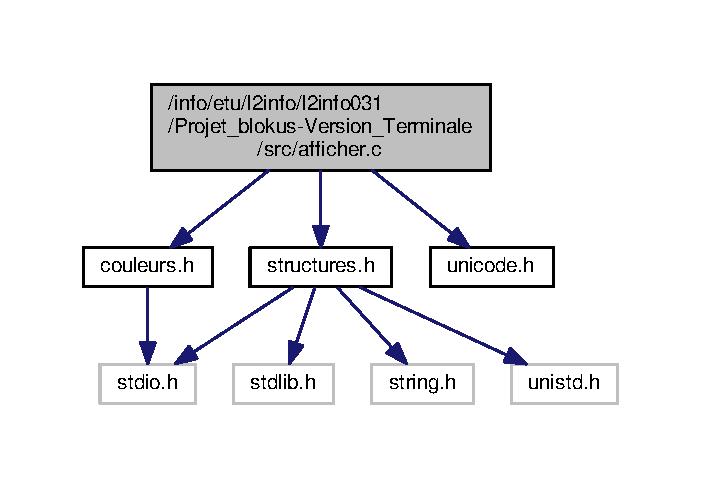
\includegraphics[width=337pt]{afficher_8c__incl}
\end{center}
\end{figure}
\subsection*{Fonctions}
\begin{DoxyCompactItemize}
\item 
void \hyperlink{afficher_8c_a68c038cdb5468dd9d574db9c08b359be}{affichage\+\_\+menu\+\_\+pause} (void)\hypertarget{afficher_8c_a68c038cdb5468dd9d574db9c08b359be}{}\label{afficher_8c_a68c038cdb5468dd9d574db9c08b359be}

\begin{DoxyCompactList}\small\item\em Affiche le menu de pause. \end{DoxyCompactList}\item 
void \hyperlink{afficher_8c_a895494ff8bb7c1a79c490a82fcb8ceb3}{affiche\+\_\+plateau} (int taille\+\_\+plateau, \hyperlink{structt__case}{t\+\_\+case}($\ast$plateau)\mbox{[}taille\+\_\+plateau\mbox{]}, int joueur, int statut, int nbj\+\_\+max)
\begin{DoxyCompactList}\small\item\em Affiche le plateau de jeu. \end{DoxyCompactList}\end{DoxyCompactItemize}


\subsection{Description détaillée}
Ensemble de fonctions d\textquotesingle{}affichage. 

\begin{DoxyAuthor}{Auteur}
Friant Marilou Tourpe Florian Semamra Kevin Amillard Joris 
\end{DoxyAuthor}
\begin{DoxyVersion}{Version}
1 
\end{DoxyVersion}


\subsection{Documentation des fonctions}
\index{afficher.\+c@{afficher.\+c}!affiche\+\_\+plateau@{affiche\+\_\+plateau}}
\index{affiche\+\_\+plateau@{affiche\+\_\+plateau}!afficher.\+c@{afficher.\+c}}
\subsubsection[{\texorpdfstring{affiche\+\_\+plateau(int taille\+\_\+plateau, t\+\_\+case($\ast$plateau)[taille\+\_\+plateau], int joueur, int statut, int nbj\+\_\+max)}{affiche_plateau(int taille_plateau, t_case(*plateau)[taille_plateau], int joueur, int statut, int nbj_max)}}]{\setlength{\rightskip}{0pt plus 5cm}void affiche\+\_\+plateau (
\begin{DoxyParamCaption}
\item[{int}]{taille\+\_\+plateau, }
\item[{{\bf t\+\_\+case}($\ast$)}]{plateau\mbox{[}taille\+\_\+plateau\mbox{]}, }
\item[{int}]{joueur, }
\item[{int}]{statut, }
\item[{int}]{nbj\+\_\+max}
\end{DoxyParamCaption}
)}\hypertarget{afficher_8c_a895494ff8bb7c1a79c490a82fcb8ceb3}{}\label{afficher_8c_a895494ff8bb7c1a79c490a82fcb8ceb3}


Affiche le plateau de jeu. 


\begin{DoxyParams}{Paramètres}
{\em taille\+\_\+plateau} & La taille du plateau \\
\hline
{\em ($\ast$plateau)\mbox{[}taille\+\_\+plateau\mbox{]}} & Le plateau \\
\hline
{\em joueur} & le joueur actuel \\
\hline
{\em nbj\+\_\+max} & Le nombre de joueurs \\
\hline
\end{DoxyParams}

\hypertarget{ajouter__piece_8c}{}\section{Référence du fichier /info/etu/l2info/l2info031/\+Projet\+\_\+blokus-\/\+Version\+\_\+\+Terminale/src/ajouter\+\_\+piece.c}
\label{ajouter__piece_8c}\index{/info/etu/l2info/l2info031/\+Projet\+\_\+blokus-\/\+Version\+\_\+\+Terminale/src/ajouter\+\_\+piece.\+c@{/info/etu/l2info/l2info031/\+Projet\+\_\+blokus-\/\+Version\+\_\+\+Terminale/src/ajouter\+\_\+piece.\+c}}


Fonctions qui vérifient le placement d\textquotesingle{}une pièce et la placent.  


{\ttfamily \#include \char`\"{}ajouter\+\_\+piece.\+h\char`\"{}}\\*
{\ttfamily \#include \char`\"{}init\+\_\+plateau.\+h\char`\"{}}\\*
Graphe des dépendances par inclusion de ajouter\+\_\+piece.\+c\+:\nopagebreak
\begin{figure}[H]
\begin{center}
\leavevmode
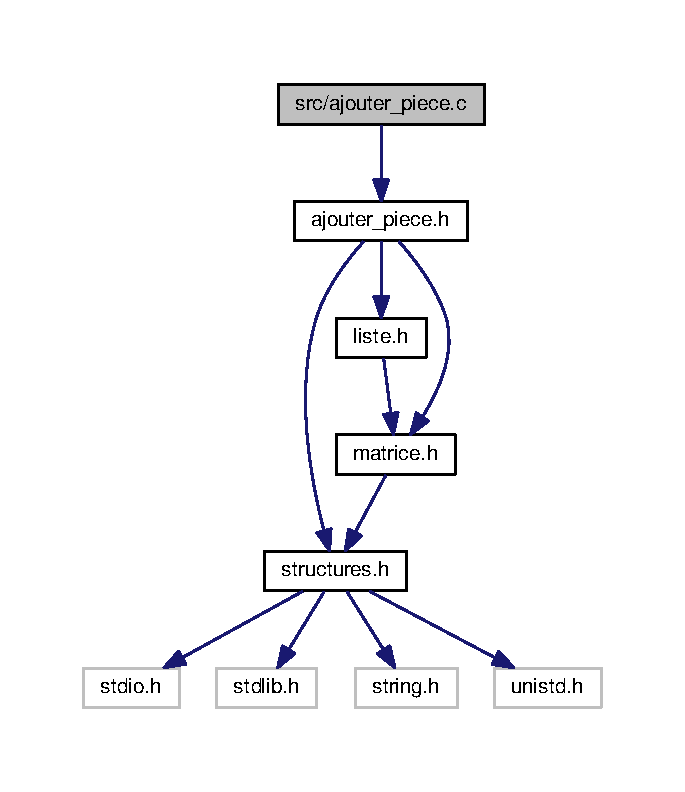
\includegraphics[width=329pt]{ajouter__piece_8c__incl}
\end{center}
\end{figure}
\subsection*{Fonctions}
\begin{DoxyCompactItemize}
\item 
void \hyperlink{ajouter__piece_8c_a76b63705ca536064dfc779ad32b1afe9}{placer\+\_\+posibiliter} (int taille\+\_\+plateau, \hyperlink{structt__case}{t\+\_\+case}($\ast$plateau)\mbox{[}taille\+\_\+plateau\mbox{]}, int y, int x, int joueur)
\begin{DoxyCompactList}\small\item\em Place dans le plateau une indication qui permet de déterminer si la case est une possibilité pour un joueur. \end{DoxyCompactList}\item 
int \hyperlink{ajouter__piece_8c_abcdf545d4b1e52e2abeb59bc45c90ffe}{placer\+\_\+piece} (int taille\+\_\+plateau, \hyperlink{structt__case}{t\+\_\+case}($\ast$plateau)\mbox{[}taille\+\_\+plateau\mbox{]}, \hyperlink{structt__matrice}{t\+\_\+matrice} matri, \hyperlink{structt__coordonnee}{t\+\_\+coordonnee} coord, int joueur, int mode)
\begin{DoxyCompactList}\small\item\em Place la pièce dans le plateau après avoir vérifié que cela soit possible. \end{DoxyCompactList}\end{DoxyCompactItemize}


\subsection{Description détaillée}
Fonctions qui vérifient le placement d\textquotesingle{}une pièce et la placent. 

\begin{DoxyAuthor}{Auteur}
Friant Marilou Tourpe Florian Semamra Kevin Amillard Joris 
\end{DoxyAuthor}
\begin{DoxyVersion}{Version}
1 
\end{DoxyVersion}


\subsection{Documentation des fonctions}
\index{ajouter\+\_\+piece.\+c@{ajouter\+\_\+piece.\+c}!placer\+\_\+piece@{placer\+\_\+piece}}
\index{placer\+\_\+piece@{placer\+\_\+piece}!ajouter\+\_\+piece.\+c@{ajouter\+\_\+piece.\+c}}
\subsubsection[{\texorpdfstring{placer\+\_\+piece(int taille\+\_\+plateau, t\+\_\+case($\ast$plateau)[taille\+\_\+plateau], t\+\_\+matrice matri, t\+\_\+coordonnee coord, int joueur, int mode)}{placer_piece(int taille_plateau, t_case(*plateau)[taille_plateau], t_matrice matri, t_coordonnee coord, int joueur, int mode)}}]{\setlength{\rightskip}{0pt plus 5cm}int placer\+\_\+piece (
\begin{DoxyParamCaption}
\item[{int}]{taille\+\_\+plateau, }
\item[{{\bf t\+\_\+case}($\ast$)}]{plateau\mbox{[}taille\+\_\+plateau\mbox{]}, }
\item[{{\bf t\+\_\+matrice}}]{matri, }
\item[{{\bf t\+\_\+coordonnee}}]{coord, }
\item[{int}]{joueur, }
\item[{int}]{mode}
\end{DoxyParamCaption}
)}\hypertarget{ajouter__piece_8c_abcdf545d4b1e52e2abeb59bc45c90ffe}{}\label{ajouter__piece_8c_abcdf545d4b1e52e2abeb59bc45c90ffe}


Place la pièce dans le plateau après avoir vérifié que cela soit possible. 


\begin{DoxyParams}{Paramètres}
{\em taille\+\_\+plateau} & la taille du plateau \\
\hline
{\em ($\ast$plateau)\mbox{[}taille\+\_\+plateau\mbox{]}} & Le plateau \\
\hline
{\em matri} & La matrice contenant la pièce \\
\hline
{\em coord} & Les coordonées de la case \\
\hline
{\em joueur} & Le joueur actuel \\
\hline
\end{DoxyParams}
\index{ajouter\+\_\+piece.\+c@{ajouter\+\_\+piece.\+c}!placer\+\_\+posibiliter@{placer\+\_\+posibiliter}}
\index{placer\+\_\+posibiliter@{placer\+\_\+posibiliter}!ajouter\+\_\+piece.\+c@{ajouter\+\_\+piece.\+c}}
\subsubsection[{\texorpdfstring{placer\+\_\+posibiliter(int taille\+\_\+plateau, t\+\_\+case($\ast$plateau)[taille\+\_\+plateau], int y, int x, int joueur)}{placer_posibiliter(int taille_plateau, t_case(*plateau)[taille_plateau], int y, int x, int joueur)}}]{\setlength{\rightskip}{0pt plus 5cm}void placer\+\_\+posibiliter (
\begin{DoxyParamCaption}
\item[{int}]{taille\+\_\+plateau, }
\item[{{\bf t\+\_\+case}($\ast$)}]{plateau\mbox{[}taille\+\_\+plateau\mbox{]}, }
\item[{int}]{y, }
\item[{int}]{x, }
\item[{int}]{joueur}
\end{DoxyParamCaption}
)}\hypertarget{ajouter__piece_8c_a76b63705ca536064dfc779ad32b1afe9}{}\label{ajouter__piece_8c_a76b63705ca536064dfc779ad32b1afe9}


Place dans le plateau une indication qui permet de déterminer si la case est une possibilité pour un joueur. 


\begin{DoxyParams}{Paramètres}
{\em taille\+\_\+plateau} & la taille du plateau \\
\hline
{\em ($\ast$plateau)\mbox{[}taille\+\_\+plateau\mbox{]}} & Le plateau \\
\hline
{\em x} & La colonne du plateau \\
\hline
{\em y} & la ligne du plateau \\
\hline
{\em joueur} & Le joueur actuel \\
\hline
\end{DoxyParams}

\hypertarget{init__plateau_8c}{}\section{init\+\_\+plateau.\+c File Reference}
\label{init__plateau_8c}\index{init\+\_\+plateau.\+c@{init\+\_\+plateau.\+c}}


Module de fonctions pour le plateau.  


{\ttfamily \#include \char`\"{}init\+\_\+plateau.\+h\char`\"{}}\newline
\subsection*{Functions}
\begin{DoxyCompactItemize}
\item 
void \mbox{\hyperlink{init__plateau_8c_aa39ae2af4a2141444eee0af667f72745}{init\+\_\+plateau}} (int taille\+\_\+plateau, \mbox{\hyperlink{structt__case}{t\+\_\+case}}($\ast$plateau)\mbox{[}taille\+\_\+plateau\mbox{]}, int nbj\+\_\+max, \mbox{\hyperlink{structt__liste}{t\+\_\+liste}} $\ast$liste\+\_\+piece, int $\ast$joueur\+\_\+en\+\_\+jeux, int $\ast$score)
\begin{DoxyCompactList}\small\item\em Initialise le plateau selon les règles du Blokus. \end{DoxyCompactList}\item 
int \mbox{\hyperlink{init__plateau_8c_a9b93825f8a4a6dd83a6a11aebc045aee}{coordonner\+\_\+invalide}} (int x, int y, int taille\+\_\+plateau)
\begin{DoxyCompactList}\small\item\em Vérifie si les coordonnées sont dans le plateau. \end{DoxyCompactList}\item 
void \mbox{\hyperlink{init__plateau_8c_adbd25dca11f18d56a22394f385a334cc}{init\+\_\+plateau\+\_\+fictif}} (int taille\+\_\+plateau, \mbox{\hyperlink{structt__case}{t\+\_\+case}}($\ast$plateau\+\_\+original)\mbox{[}taille\+\_\+plateau\mbox{]}, \mbox{\hyperlink{structt__case}{t\+\_\+case}}($\ast$plateau\+\_\+copie)\mbox{[}taille\+\_\+plateau\mbox{]}, int joueur, \mbox{\hyperlink{structt__coordonnee}{t\+\_\+coordonnee}} $\ast$coord)
\begin{DoxyCompactList}\small\item\em Créé un plateau avec une seule possibilité de placement. \end{DoxyCompactList}\item 
void \mbox{\hyperlink{init__plateau_8c_ac05e76e09561c2c6fdf47c4bab1f7c3a}{copie\+\_\+plateau}} (int taille\+\_\+plateau, \mbox{\hyperlink{structt__case}{t\+\_\+case}}($\ast$plateau\+\_\+original)\mbox{[}taille\+\_\+plateau\mbox{]}, \mbox{\hyperlink{structt__case}{t\+\_\+case}}($\ast$plateau\+\_\+copie)\mbox{[}taille\+\_\+plateau\mbox{]})
\begin{DoxyCompactList}\small\item\em Copie le tableau dans un autrre. \end{DoxyCompactList}\end{DoxyCompactItemize}


\subsection{Detailed Description}
Module de fonctions pour le plateau. 

\begin{DoxyAuthor}{Author}
Friant Marilou Tourpe Florian Semamra Kevin Amillard Joris 
\end{DoxyAuthor}
\begin{DoxyVersion}{Version}
1 
\end{DoxyVersion}


\subsection{Function Documentation}
\mbox{\Hypertarget{init__plateau_8c_a9b93825f8a4a6dd83a6a11aebc045aee}\label{init__plateau_8c_a9b93825f8a4a6dd83a6a11aebc045aee}} 
\index{init\+\_\+plateau.\+c@{init\+\_\+plateau.\+c}!coordonner\+\_\+invalide@{coordonner\+\_\+invalide}}
\index{coordonner\+\_\+invalide@{coordonner\+\_\+invalide}!init\+\_\+plateau.\+c@{init\+\_\+plateau.\+c}}
\subsubsection{\texorpdfstring{coordonner\+\_\+invalide()}{coordonner\_invalide()}}
{\footnotesize\ttfamily int coordonner\+\_\+invalide (\begin{DoxyParamCaption}\item[{int}]{x,  }\item[{int}]{y,  }\item[{int}]{taille\+\_\+plateau }\end{DoxyParamCaption})}



Vérifie si les coordonnées sont dans le plateau. 


\begin{DoxyParams}{Parameters}
{\em x} & La colonne du plateau \\
\hline
{\em y} & La ligne du plateau \\
\hline
{\em taille\+\_\+plateau} & la aille du plateau \\
\hline
\end{DoxyParams}
\mbox{\Hypertarget{init__plateau_8c_ac05e76e09561c2c6fdf47c4bab1f7c3a}\label{init__plateau_8c_ac05e76e09561c2c6fdf47c4bab1f7c3a}} 
\index{init\+\_\+plateau.\+c@{init\+\_\+plateau.\+c}!copie\+\_\+plateau@{copie\+\_\+plateau}}
\index{copie\+\_\+plateau@{copie\+\_\+plateau}!init\+\_\+plateau.\+c@{init\+\_\+plateau.\+c}}
\subsubsection{\texorpdfstring{copie\+\_\+plateau()}{copie\_plateau()}}
{\footnotesize\ttfamily void copie\+\_\+plateau (\begin{DoxyParamCaption}\item[{int}]{taille\+\_\+plateau,  }\item[{\mbox{\hyperlink{structt__case}{t\+\_\+case}}($\ast$)}]{plateau\+\_\+original\mbox{[}taille\+\_\+plateau\mbox{]},  }\item[{\mbox{\hyperlink{structt__case}{t\+\_\+case}}($\ast$)}]{plateau\+\_\+copie\mbox{[}taille\+\_\+plateau\mbox{]} }\end{DoxyParamCaption})}



Copie le tableau dans un autrre. 


\begin{DoxyParams}{Parameters}
{\em taille\+\_\+plateau} & La taille du plateau \\
\hline
{\em ($\ast$plateau\+\_\+original)\mbox{[}taille\+\_\+plateau\mbox{]}} & Le plateau original \\
\hline
{\em ($\ast$plateau\+\_\+copie)\mbox{[}taille\+\_\+plateau\mbox{]}} & Le plateau copié \\
\hline
\end{DoxyParams}
\mbox{\Hypertarget{init__plateau_8c_aa39ae2af4a2141444eee0af667f72745}\label{init__plateau_8c_aa39ae2af4a2141444eee0af667f72745}} 
\index{init\+\_\+plateau.\+c@{init\+\_\+plateau.\+c}!init\+\_\+plateau@{init\+\_\+plateau}}
\index{init\+\_\+plateau@{init\+\_\+plateau}!init\+\_\+plateau.\+c@{init\+\_\+plateau.\+c}}
\subsubsection{\texorpdfstring{init\+\_\+plateau()}{init\_plateau()}}
{\footnotesize\ttfamily void init\+\_\+plateau (\begin{DoxyParamCaption}\item[{int}]{taille\+\_\+plateau,  }\item[{\mbox{\hyperlink{structt__case}{t\+\_\+case}}($\ast$)}]{plateau\mbox{[}taille\+\_\+plateau\mbox{]},  }\item[{int}]{nbj\+\_\+max,  }\item[{\mbox{\hyperlink{structt__liste}{t\+\_\+liste}} $\ast$}]{liste\+\_\+piece,  }\item[{int $\ast$}]{joueur\+\_\+en\+\_\+jeux,  }\item[{int $\ast$}]{score }\end{DoxyParamCaption})}



Initialise le plateau selon les règles du Blokus. 


\begin{DoxyParams}{Parameters}
{\em taille\+\_\+plateau} & la taille du plateau \\
\hline
{\em ($\ast$plateau)\mbox{[}taille\+\_\+plateau\mbox{]}} & Le plateau \\
\hline
{\em nbj\+\_\+max} & Le nombre de joueurs \\
\hline
{\em $\ast$liste} & Pointeur sur une liste de pièces \\
\hline
{\em $\ast$joueurs\+\_\+en\+\_\+jeux} & Le nombre de joueurs encore en jeu \\
\hline
{\em $\ast$score} & Le score de chaque joueur \\
\hline
\end{DoxyParams}
\mbox{\Hypertarget{init__plateau_8c_adbd25dca11f18d56a22394f385a334cc}\label{init__plateau_8c_adbd25dca11f18d56a22394f385a334cc}} 
\index{init\+\_\+plateau.\+c@{init\+\_\+plateau.\+c}!init\+\_\+plateau\+\_\+fictif@{init\+\_\+plateau\+\_\+fictif}}
\index{init\+\_\+plateau\+\_\+fictif@{init\+\_\+plateau\+\_\+fictif}!init\+\_\+plateau.\+c@{init\+\_\+plateau.\+c}}
\subsubsection{\texorpdfstring{init\+\_\+plateau\+\_\+fictif()}{init\_plateau\_fictif()}}
{\footnotesize\ttfamily void init\+\_\+plateau\+\_\+fictif (\begin{DoxyParamCaption}\item[{int}]{taille\+\_\+plateau,  }\item[{\mbox{\hyperlink{structt__case}{t\+\_\+case}}($\ast$)}]{plateau\+\_\+original\mbox{[}taille\+\_\+plateau\mbox{]},  }\item[{\mbox{\hyperlink{structt__case}{t\+\_\+case}}($\ast$)}]{plateau\+\_\+copie\mbox{[}taille\+\_\+plateau\mbox{]},  }\item[{int}]{joueur,  }\item[{\mbox{\hyperlink{structt__coordonnee}{t\+\_\+coordonnee}} $\ast$}]{coord }\end{DoxyParamCaption})}



Créé un plateau avec une seule possibilité de placement. 


\begin{DoxyParams}{Parameters}
{\em taille\+\_\+plateau} & la taille du plateau \\
\hline
{\em ($\ast$plateau)\mbox{[}taille\+\_\+plateau\mbox{]}} & Le plateau \\
\hline
{\em nbj\+\_\+max} & Le nombre de joueurs \\
\hline
{\em $\ast$liste} & Pointeur sur une liste de pièces \\
\hline
{\em $\ast$joueurs\+\_\+en\+\_\+jeux} & Le nombre de joueurs encore en jeu \\
\hline
{\em $\ast$score} & Le score de chaque joueur \\
\hline
\end{DoxyParams}

\hypertarget{liste_8c}{}\section{Référence du fichier src/liste.c}
\label{liste_8c}\index{src/liste.\+c@{src/liste.\+c}}


Ensemble de fonctions servants � l\textquotesingle{}utilisation des listes.  


{\ttfamily \#include \char`\"{}liste.\+h\char`\"{}}\\*
Graphe des dépendances par inclusion de liste.\+c\+:
\nopagebreak
\begin{figure}[H]
\begin{center}
\leavevmode
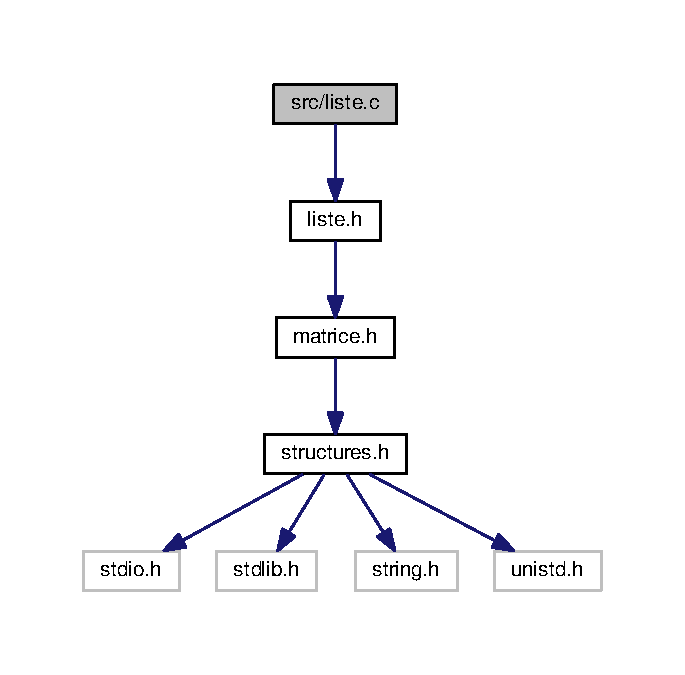
\includegraphics[width=329pt]{liste_8c__incl}
\end{center}
\end{figure}
\subsection*{Fonctions}
\begin{DoxyCompactItemize}
\item 
void \hyperlink{liste_8c_a5cc83f8eeeb903a8b631ef84f9efffcf}{copie\+\_\+liste} (int nbj\+\_\+max, \hyperlink{structt__liste}{t\+\_\+liste} source\mbox{[}nbj\+\_\+max\mbox{]}, \hyperlink{structt__liste}{t\+\_\+liste} copie\mbox{[}nbj\+\_\+max\mbox{]})
\begin{DoxyCompactList}\small\item\em Fonction qui copie une liste source sur la liste copie. \end{DoxyCompactList}\item 
void \hyperlink{liste_8c_a7dda997062b284703a6637cb25a8871a}{init\+\_\+liste} (\hyperlink{structt__liste}{t\+\_\+liste} $\ast$liste)
\begin{DoxyCompactList}\small\item\em Initialise la liste. \end{DoxyCompactList}\item 
int \hyperlink{liste_8c_aaf6d7622b271b1fba9c0eb73a5d6db44}{liste\+\_\+vide} (\hyperlink{structt__liste}{t\+\_\+liste} $\ast$liste)
\begin{DoxyCompactList}\small\item\em Indique si une liste est vide ou non. \end{DoxyCompactList}\item 
int \hyperlink{liste_8c_a1ec9a3419a08cb571c722eb8eeb45224}{hors\+\_\+liste} (\hyperlink{structt__liste}{t\+\_\+liste} $\ast$liste)
\begin{DoxyCompactList}\small\item\em Indique si l\textquotesingle{}�l�ment courant de la liste se trouve bien dans la liste. \end{DoxyCompactList}\item 
void \hyperlink{liste_8c_a6f3dc42709b31e9eb527e3018568e766}{en\+\_\+tete} (\hyperlink{structt__liste}{t\+\_\+liste} $\ast$liste)
\begin{DoxyCompactList}\small\item\em Fonction qui place l\textquotesingle{}�l�ment courant en t�te de liste. \end{DoxyCompactList}\item 
void \hyperlink{liste_8c_a0070ce853ee19eac4f1226988a494e01}{en\+\_\+queue} (\hyperlink{structt__liste}{t\+\_\+liste} $\ast$liste)
\begin{DoxyCompactList}\small\item\em Fonction qui place l\textquotesingle{}�l�ment courant en queue de liste. \end{DoxyCompactList}\item 
void \hyperlink{liste_8c_a8e2e7a55e996e294e79a6e607cad00dc}{precedent} (\hyperlink{structt__liste}{t\+\_\+liste} $\ast$liste)
\begin{DoxyCompactList}\small\item\em Fonction qui place l\textquotesingle{}�l�ment courant sur l\textquotesingle{}�l�ment pr�c�dent. \end{DoxyCompactList}\item 
void \hyperlink{liste_8c_ac76a08dfdd4e447188d85378a1c39aba}{suivant} (\hyperlink{structt__liste}{t\+\_\+liste} $\ast$liste)
\begin{DoxyCompactList}\small\item\em Fonction qui place l\textquotesingle{}�l�ment courant sur l\textquotesingle{}�l�ment suivant. \end{DoxyCompactList}\item 
void \hyperlink{liste_8c_a24e91e6bd38de3d8e043dd079256053b}{val\+\_\+elem} (\hyperlink{structt__liste}{t\+\_\+liste} $\ast$liste, \hyperlink{structt__matrice}{t\+\_\+matrice} $\ast$copie)
\begin{DoxyCompactList}\small\item\em Fonction qui r�cup�re la matrice de l\textquotesingle{}�l�ment courant et la copie. \end{DoxyCompactList}\item 
void \hyperlink{liste_8c_a6173fcd0d246aa6ab73cfd9395d1e179}{oter\+\_\+elt} (\hyperlink{structt__liste}{t\+\_\+liste} $\ast$liste)
\begin{DoxyCompactList}\small\item\em Fonction qui supprime l\textquotesingle{}�l�ment courant. \end{DoxyCompactList}\item 
void \hyperlink{liste_8c_a3fcc34a240ac672285b9588bb8c6c1ec}{placer\+\_\+elem} (\hyperlink{structt__liste}{t\+\_\+liste} $\ast$liste, \hyperlink{structt__matrice}{t\+\_\+matrice} $\ast$piece)
\begin{DoxyCompactList}\small\item\em Fonction qui place ou remplace une matrice dans la liste. \end{DoxyCompactList}\item 
void \hyperlink{liste_8c_a08a7b02c46805f275729f5639551f144}{ajouter\+\_\+piece} (\hyperlink{structt__liste}{t\+\_\+liste} $\ast$liste, \hyperlink{structt__matrice}{t\+\_\+matrice} $\ast$piece)
\begin{DoxyCompactList}\small\item\em Fonction qui place une pi�ce au bon endroit de la liste. \end{DoxyCompactList}\item 
void \hyperlink{liste_8c_a13b2afdaa5eec613cf6d42eb49eae08a}{remplir\+\_\+listes} (\hyperlink{structt__liste}{t\+\_\+liste} $\ast$liste)
\begin{DoxyCompactList}\small\item\em Fonction qui remplit une liste avec une banque de pi�ces contenue dans un fichier. \end{DoxyCompactList}\end{DoxyCompactItemize}


\subsection{Description détaillée}
Ensemble de fonctions servants � l\textquotesingle{}utilisation des listes. 

\begin{DoxyAuthor}{Auteur}
Friant Marilou Tourpe Florian Semamra Kevin Amillard Joris 
\end{DoxyAuthor}
\begin{DoxyVersion}{Version}
1 
\end{DoxyVersion}


\subsection{Documentation des fonctions}
\index{liste.\+c@{liste.\+c}!ajouter\+\_\+piece@{ajouter\+\_\+piece}}
\index{ajouter\+\_\+piece@{ajouter\+\_\+piece}!liste.\+c@{liste.\+c}}
\subsubsection[{\texorpdfstring{ajouter\+\_\+piece(t\+\_\+liste $\ast$liste, t\+\_\+matrice $\ast$piece)}{ajouter_piece(t_liste *liste, t_matrice *piece)}}]{\setlength{\rightskip}{0pt plus 5cm}void ajouter\+\_\+piece (
\begin{DoxyParamCaption}
\item[{{\bf t\+\_\+liste} $\ast$}]{liste, }
\item[{{\bf t\+\_\+matrice} $\ast$}]{piece}
\end{DoxyParamCaption}
)}\hypertarget{liste_8c_a08a7b02c46805f275729f5639551f144}{}\label{liste_8c_a08a7b02c46805f275729f5639551f144}


Fonction qui place une pi�ce au bon endroit de la liste. 


\begin{DoxyParams}{Paramètres}
{\em $\ast$liste} & La liste \\
\hline
{\em $\ast$piece} & La pi�ce \\
\hline
\end{DoxyParams}
\index{liste.\+c@{liste.\+c}!copie\+\_\+liste@{copie\+\_\+liste}}
\index{copie\+\_\+liste@{copie\+\_\+liste}!liste.\+c@{liste.\+c}}
\subsubsection[{\texorpdfstring{copie\+\_\+liste(int nbj\+\_\+max, t\+\_\+liste source[nbj\+\_\+max], t\+\_\+liste copie[nbj\+\_\+max])}{copie_liste(int nbj_max, t_liste source[nbj_max], t_liste copie[nbj_max])}}]{\setlength{\rightskip}{0pt plus 5cm}void copie\+\_\+liste (
\begin{DoxyParamCaption}
\item[{int}]{nbj\+\_\+max, }
\item[{{\bf t\+\_\+liste}}]{source\mbox{[}nbj\+\_\+max\mbox{]}, }
\item[{{\bf t\+\_\+liste}}]{copie\mbox{[}nbj\+\_\+max\mbox{]}}
\end{DoxyParamCaption}
)}\hypertarget{liste_8c_a5cc83f8eeeb903a8b631ef84f9efffcf}{}\label{liste_8c_a5cc83f8eeeb903a8b631ef84f9efffcf}


Fonction qui copie une liste source sur la liste copie. 


\begin{DoxyParams}{Paramètres}
{\em nbj\+\_\+max} & Nombre de joueur dans la partie \\
\hline
{\em source\mbox{[}nbj\+\_\+max\mbox{]}} & La source \\
\hline
{\em copie\mbox{[}nbj\+\_\+max\mbox{]}} & La copie \\
\hline
\end{DoxyParams}
\index{liste.\+c@{liste.\+c}!en\+\_\+queue@{en\+\_\+queue}}
\index{en\+\_\+queue@{en\+\_\+queue}!liste.\+c@{liste.\+c}}
\subsubsection[{\texorpdfstring{en\+\_\+queue(t\+\_\+liste $\ast$liste)}{en_queue(t_liste *liste)}}]{\setlength{\rightskip}{0pt plus 5cm}void en\+\_\+queue (
\begin{DoxyParamCaption}
\item[{{\bf t\+\_\+liste} $\ast$}]{liste}
\end{DoxyParamCaption}
)}\hypertarget{liste_8c_a0070ce853ee19eac4f1226988a494e01}{}\label{liste_8c_a0070ce853ee19eac4f1226988a494e01}


Fonction qui place l\textquotesingle{}�l�ment courant en queue de liste. 


\begin{DoxyParams}{Paramètres}
{\em $\ast$liste} & La liste \\
\hline
\end{DoxyParams}
\index{liste.\+c@{liste.\+c}!en\+\_\+tete@{en\+\_\+tete}}
\index{en\+\_\+tete@{en\+\_\+tete}!liste.\+c@{liste.\+c}}
\subsubsection[{\texorpdfstring{en\+\_\+tete(t\+\_\+liste $\ast$liste)}{en_tete(t_liste *liste)}}]{\setlength{\rightskip}{0pt plus 5cm}void en\+\_\+tete (
\begin{DoxyParamCaption}
\item[{{\bf t\+\_\+liste} $\ast$}]{liste}
\end{DoxyParamCaption}
)}\hypertarget{liste_8c_a6f3dc42709b31e9eb527e3018568e766}{}\label{liste_8c_a6f3dc42709b31e9eb527e3018568e766}


Fonction qui place l\textquotesingle{}�l�ment courant en t�te de liste. 


\begin{DoxyParams}{Paramètres}
{\em $\ast$liste} & La liste \\
\hline
\end{DoxyParams}
\index{liste.\+c@{liste.\+c}!hors\+\_\+liste@{hors\+\_\+liste}}
\index{hors\+\_\+liste@{hors\+\_\+liste}!liste.\+c@{liste.\+c}}
\subsubsection[{\texorpdfstring{hors\+\_\+liste(t\+\_\+liste $\ast$liste)}{hors_liste(t_liste *liste)}}]{\setlength{\rightskip}{0pt plus 5cm}int hors\+\_\+liste (
\begin{DoxyParamCaption}
\item[{{\bf t\+\_\+liste} $\ast$}]{liste}
\end{DoxyParamCaption}
)}\hypertarget{liste_8c_a1ec9a3419a08cb571c722eb8eeb45224}{}\label{liste_8c_a1ec9a3419a08cb571c722eb8eeb45224}


Indique si l\textquotesingle{}�l�ment courant de la liste se trouve bien dans la liste. 


\begin{DoxyParams}{Paramètres}
{\em $\ast$liste} & La liste \\
\hline
\end{DoxyParams}
\index{liste.\+c@{liste.\+c}!init\+\_\+liste@{init\+\_\+liste}}
\index{init\+\_\+liste@{init\+\_\+liste}!liste.\+c@{liste.\+c}}
\subsubsection[{\texorpdfstring{init\+\_\+liste(t\+\_\+liste $\ast$liste)}{init_liste(t_liste *liste)}}]{\setlength{\rightskip}{0pt plus 5cm}void init\+\_\+liste (
\begin{DoxyParamCaption}
\item[{{\bf t\+\_\+liste} $\ast$}]{liste}
\end{DoxyParamCaption}
)}\hypertarget{liste_8c_a7dda997062b284703a6637cb25a8871a}{}\label{liste_8c_a7dda997062b284703a6637cb25a8871a}


Initialise la liste. 


\begin{DoxyParams}{Paramètres}
{\em $\ast$liste} & La liste \\
\hline
\end{DoxyParams}
\index{liste.\+c@{liste.\+c}!liste\+\_\+vide@{liste\+\_\+vide}}
\index{liste\+\_\+vide@{liste\+\_\+vide}!liste.\+c@{liste.\+c}}
\subsubsection[{\texorpdfstring{liste\+\_\+vide(t\+\_\+liste $\ast$liste)}{liste_vide(t_liste *liste)}}]{\setlength{\rightskip}{0pt plus 5cm}int liste\+\_\+vide (
\begin{DoxyParamCaption}
\item[{{\bf t\+\_\+liste} $\ast$}]{liste}
\end{DoxyParamCaption}
)}\hypertarget{liste_8c_aaf6d7622b271b1fba9c0eb73a5d6db44}{}\label{liste_8c_aaf6d7622b271b1fba9c0eb73a5d6db44}


Indique si une liste est vide ou non. 


\begin{DoxyParams}{Paramètres}
{\em $\ast$liste} & La liste \\
\hline
\end{DoxyParams}
\index{liste.\+c@{liste.\+c}!oter\+\_\+elt@{oter\+\_\+elt}}
\index{oter\+\_\+elt@{oter\+\_\+elt}!liste.\+c@{liste.\+c}}
\subsubsection[{\texorpdfstring{oter\+\_\+elt(t\+\_\+liste $\ast$liste)}{oter_elt(t_liste *liste)}}]{\setlength{\rightskip}{0pt plus 5cm}void oter\+\_\+elt (
\begin{DoxyParamCaption}
\item[{{\bf t\+\_\+liste} $\ast$}]{liste}
\end{DoxyParamCaption}
)}\hypertarget{liste_8c_a6173fcd0d246aa6ab73cfd9395d1e179}{}\label{liste_8c_a6173fcd0d246aa6ab73cfd9395d1e179}


Fonction qui supprime l\textquotesingle{}�l�ment courant. 


\begin{DoxyParams}{Paramètres}
{\em $\ast$liste} & La liste \\
\hline
\end{DoxyParams}
\index{liste.\+c@{liste.\+c}!placer\+\_\+elem@{placer\+\_\+elem}}
\index{placer\+\_\+elem@{placer\+\_\+elem}!liste.\+c@{liste.\+c}}
\subsubsection[{\texorpdfstring{placer\+\_\+elem(t\+\_\+liste $\ast$liste, t\+\_\+matrice $\ast$piece)}{placer_elem(t_liste *liste, t_matrice *piece)}}]{\setlength{\rightskip}{0pt plus 5cm}void placer\+\_\+elem (
\begin{DoxyParamCaption}
\item[{{\bf t\+\_\+liste} $\ast$}]{liste, }
\item[{{\bf t\+\_\+matrice} $\ast$}]{piece}
\end{DoxyParamCaption}
)}\hypertarget{liste_8c_a3fcc34a240ac672285b9588bb8c6c1ec}{}\label{liste_8c_a3fcc34a240ac672285b9588bb8c6c1ec}


Fonction qui place ou remplace une matrice dans la liste. 


\begin{DoxyParams}{Paramètres}
{\em $\ast$liste} & La liste \\
\hline
{\em $\ast$piece} & La pi�ce \\
\hline
\end{DoxyParams}
\index{liste.\+c@{liste.\+c}!precedent@{precedent}}
\index{precedent@{precedent}!liste.\+c@{liste.\+c}}
\subsubsection[{\texorpdfstring{precedent(t\+\_\+liste $\ast$liste)}{precedent(t_liste *liste)}}]{\setlength{\rightskip}{0pt plus 5cm}void precedent (
\begin{DoxyParamCaption}
\item[{{\bf t\+\_\+liste} $\ast$}]{liste}
\end{DoxyParamCaption}
)}\hypertarget{liste_8c_a8e2e7a55e996e294e79a6e607cad00dc}{}\label{liste_8c_a8e2e7a55e996e294e79a6e607cad00dc}


Fonction qui place l\textquotesingle{}�l�ment courant sur l\textquotesingle{}�l�ment pr�c�dent. 


\begin{DoxyParams}{Paramètres}
{\em $\ast$liste} & La liste \\
\hline
\end{DoxyParams}
\index{liste.\+c@{liste.\+c}!remplir\+\_\+listes@{remplir\+\_\+listes}}
\index{remplir\+\_\+listes@{remplir\+\_\+listes}!liste.\+c@{liste.\+c}}
\subsubsection[{\texorpdfstring{remplir\+\_\+listes(t\+\_\+liste $\ast$liste)}{remplir_listes(t_liste *liste)}}]{\setlength{\rightskip}{0pt plus 5cm}void remplir\+\_\+listes (
\begin{DoxyParamCaption}
\item[{{\bf t\+\_\+liste} $\ast$}]{liste}
\end{DoxyParamCaption}
)}\hypertarget{liste_8c_a13b2afdaa5eec613cf6d42eb49eae08a}{}\label{liste_8c_a13b2afdaa5eec613cf6d42eb49eae08a}


Fonction qui remplit une liste avec une banque de pi�ces contenue dans un fichier. 


\begin{DoxyParams}{Paramètres}
{\em $\ast$liste} & La liste \\
\hline
\end{DoxyParams}
\index{liste.\+c@{liste.\+c}!suivant@{suivant}}
\index{suivant@{suivant}!liste.\+c@{liste.\+c}}
\subsubsection[{\texorpdfstring{suivant(t\+\_\+liste $\ast$liste)}{suivant(t_liste *liste)}}]{\setlength{\rightskip}{0pt plus 5cm}void suivant (
\begin{DoxyParamCaption}
\item[{{\bf t\+\_\+liste} $\ast$}]{liste}
\end{DoxyParamCaption}
)}\hypertarget{liste_8c_ac76a08dfdd4e447188d85378a1c39aba}{}\label{liste_8c_ac76a08dfdd4e447188d85378a1c39aba}


Fonction qui place l\textquotesingle{}�l�ment courant sur l\textquotesingle{}�l�ment suivant. 


\begin{DoxyParams}{Paramètres}
{\em $\ast$liste} & La liste \\
\hline
\end{DoxyParams}
\index{liste.\+c@{liste.\+c}!val\+\_\+elem@{val\+\_\+elem}}
\index{val\+\_\+elem@{val\+\_\+elem}!liste.\+c@{liste.\+c}}
\subsubsection[{\texorpdfstring{val\+\_\+elem(t\+\_\+liste $\ast$liste, t\+\_\+matrice $\ast$copie)}{val_elem(t_liste *liste, t_matrice *copie)}}]{\setlength{\rightskip}{0pt plus 5cm}void val\+\_\+elem (
\begin{DoxyParamCaption}
\item[{{\bf t\+\_\+liste} $\ast$}]{liste, }
\item[{{\bf t\+\_\+matrice} $\ast$}]{copie}
\end{DoxyParamCaption}
)}\hypertarget{liste_8c_a24e91e6bd38de3d8e043dd079256053b}{}\label{liste_8c_a24e91e6bd38de3d8e043dd079256053b}


Fonction qui r�cup�re la matrice de l\textquotesingle{}�l�ment courant et la copie. 


\begin{DoxyParams}{Paramètres}
{\em $\ast$liste} & La liste \\
\hline
{\em $\ast$copie} & La matrice contenant la copie \\
\hline
\end{DoxyParams}

\hypertarget{menu__pause_8c}{}\section{menu\+\_\+pause.\+c File Reference}
\label{menu__pause_8c}\index{menu\+\_\+pause.\+c@{menu\+\_\+pause.\+c}}


Fonctions de sauvegarde, de chargement et du menu de pause.  


{\ttfamily \#include \char`\"{}menu\+\_\+pause.\+h\char`\"{}}\newline
{\ttfamily \#include \char`\"{}Partie.\+h\char`\"{}}\newline
{\ttfamily \#include \char`\"{}afficher.\+h\char`\"{}}\newline
\subsection*{Functions}
\begin{DoxyCompactItemize}
\item 
\mbox{\Hypertarget{menu__pause_8c_a567460c4b8ba2212718aabec861b1942}\label{menu__pause_8c_a567460c4b8ba2212718aabec861b1942}} 
int \mbox{\hyperlink{menu__pause_8c_a567460c4b8ba2212718aabec861b1942}{charger\+\_\+partie}} ()
\begin{DoxyCompactList}\small\item\em Charge une partie � partir d\textquotesingle{}un fichier de sauvegarde. \end{DoxyCompactList}\item 
void \mbox{\hyperlink{menu__pause_8c_ab457b68b014d212a7422799f111e0a1e}{sauvegarder\+\_\+partie}} (int nbj, int nbj\+\_\+max, int nb\+\_\+tour\+\_\+joueur, int $\ast$score, int $\ast$player, int taille\+\_\+plateau, \mbox{\hyperlink{structt__case}{t\+\_\+case}}($\ast$plateau)\mbox{[}taille\+\_\+plateau\mbox{]}, \mbox{\hyperlink{structt__liste}{t\+\_\+liste}} $\ast$liste\+\_\+piece)
\begin{DoxyCompactList}\small\item\em Sauvegarde la partie. \end{DoxyCompactList}\item 
int \mbox{\hyperlink{menu__pause_8c_aa1170c11785fa53547eb25ff34af4fbd}{menu\+\_\+pause}} (int nbj, int nbj\+\_\+max, int nb\+\_\+tour\+\_\+joueur, int $\ast$score, int $\ast$player, int taille\+\_\+plateau, \mbox{\hyperlink{structt__case}{t\+\_\+case}}($\ast$plateau)\mbox{[}taille\+\_\+plateau\mbox{]}, \mbox{\hyperlink{structt__liste}{t\+\_\+liste}} $\ast$liste\+\_\+piece)
\begin{DoxyCompactList}\small\item\em Le menu de pause. \end{DoxyCompactList}\end{DoxyCompactItemize}


\subsection{Detailed Description}
Fonctions de sauvegarde, de chargement et du menu de pause. 

\begin{DoxyAuthor}{Author}
Friant Marilou Tourpe Florian Semamra Kevin Amillard Joris 
\end{DoxyAuthor}
\begin{DoxyVersion}{Version}
1 
\end{DoxyVersion}


\subsection{Function Documentation}
\mbox{\Hypertarget{menu__pause_8c_aa1170c11785fa53547eb25ff34af4fbd}\label{menu__pause_8c_aa1170c11785fa53547eb25ff34af4fbd}} 
\index{menu\+\_\+pause.\+c@{menu\+\_\+pause.\+c}!menu\+\_\+pause@{menu\+\_\+pause}}
\index{menu\+\_\+pause@{menu\+\_\+pause}!menu\+\_\+pause.\+c@{menu\+\_\+pause.\+c}}
\subsubsection{\texorpdfstring{menu\+\_\+pause()}{menu\_pause()}}
{\footnotesize\ttfamily menu\+\_\+pause (\begin{DoxyParamCaption}\item[{int}]{nbj,  }\item[{int}]{nbj\+\_\+max,  }\item[{int}]{nb\+\_\+tour\+\_\+joueur,  }\item[{int $\ast$}]{score,  }\item[{int $\ast$}]{player,  }\item[{int}]{taille\+\_\+plateau,  }\item[{\mbox{\hyperlink{structt__case}{t\+\_\+case}}($\ast$)}]{plateau\mbox{[}taille\+\_\+plateau\mbox{]},  }\item[{\mbox{\hyperlink{structt__liste}{t\+\_\+liste}} $\ast$}]{liste\+\_\+piece }\end{DoxyParamCaption})}



Le menu de pause. 


\begin{DoxyParams}{Parameters}
{\em nbj} & Nombre de joueurs ordinateurs \\
\hline
{\em nbj\+\_\+max} & Nombre de joueurs \\
\hline
{\em nb\+\_\+tour\+\_\+joueur} & Le tour \\
\hline
{\em $\ast$score} & Tableau des scores des joueurs \\
\hline
{\em $\ast$player} & \\
\hline
{\em taille\+\_\+plateau} & La taille du plateau \\
\hline
{\em ($\ast$plateau)\mbox{[}taille\+\_\+plateau\mbox{]}} & Le plateau \\
\hline
{\em $\ast$liste\+\_\+piece} & Les listes de pi�ces des joueurs \\
\hline
\end{DoxyParams}
\mbox{\Hypertarget{menu__pause_8c_ab457b68b014d212a7422799f111e0a1e}\label{menu__pause_8c_ab457b68b014d212a7422799f111e0a1e}} 
\index{menu\+\_\+pause.\+c@{menu\+\_\+pause.\+c}!sauvegarder\+\_\+partie@{sauvegarder\+\_\+partie}}
\index{sauvegarder\+\_\+partie@{sauvegarder\+\_\+partie}!menu\+\_\+pause.\+c@{menu\+\_\+pause.\+c}}
\subsubsection{\texorpdfstring{sauvegarder\+\_\+partie()}{sauvegarder\_partie()}}
{\footnotesize\ttfamily void sauvegarder\+\_\+partie (\begin{DoxyParamCaption}\item[{int}]{nbj,  }\item[{int}]{nbj\+\_\+max,  }\item[{int}]{nb\+\_\+tour\+\_\+joueur,  }\item[{int $\ast$}]{score,  }\item[{int $\ast$}]{player,  }\item[{int}]{taille\+\_\+plateau,  }\item[{\mbox{\hyperlink{structt__case}{t\+\_\+case}}($\ast$)}]{plateau\mbox{[}taille\+\_\+plateau\mbox{]},  }\item[{\mbox{\hyperlink{structt__liste}{t\+\_\+liste}} $\ast$}]{liste\+\_\+piece }\end{DoxyParamCaption})}



Sauvegarde la partie. 

Enregistre dans un fichier l\textquotesingle{}�tat du plateau, les pi�ces restantes de chaque joueur ainsi que leur score et � qui c\textquotesingle{}est le tour de jouer 
\begin{DoxyParams}{Parameters}
{\em nbj} & Nombre de joueurs ordinateurs \\
\hline
{\em nbj\+\_\+max} & Nombre de joueurs \\
\hline
{\em nb\+\_\+tour\+\_\+joueur} & Le tour \\
\hline
{\em $\ast$score} & Tableau des scores des joueurs \\
\hline
{\em $\ast$player} & \\
\hline
{\em taille\+\_\+plateau} & La taille du plateau \\
\hline
{\em ($\ast$plateau)\mbox{[}taille\+\_\+plateau\mbox{]}} & Le plateau \\
\hline
{\em $\ast$liste\+\_\+piece} & Les listes de pi�ces des joueurs \\
\hline
\end{DoxyParams}

\hypertarget{Partie_8c}{}\section{Référence du fichier src/\+Partie.c}
\label{Partie_8c}\index{src/\+Partie.\+c@{src/\+Partie.\+c}}


Ensemble de fonctions qui font tourner une partie de jeu. Fichier principal.  


{\ttfamily \#include \char`\"{}Partie.\+h\char`\"{}}\\*
Graphe des dépendances par inclusion de Partie.\+c\+:
\nopagebreak
\begin{figure}[H]
\begin{center}
\leavevmode
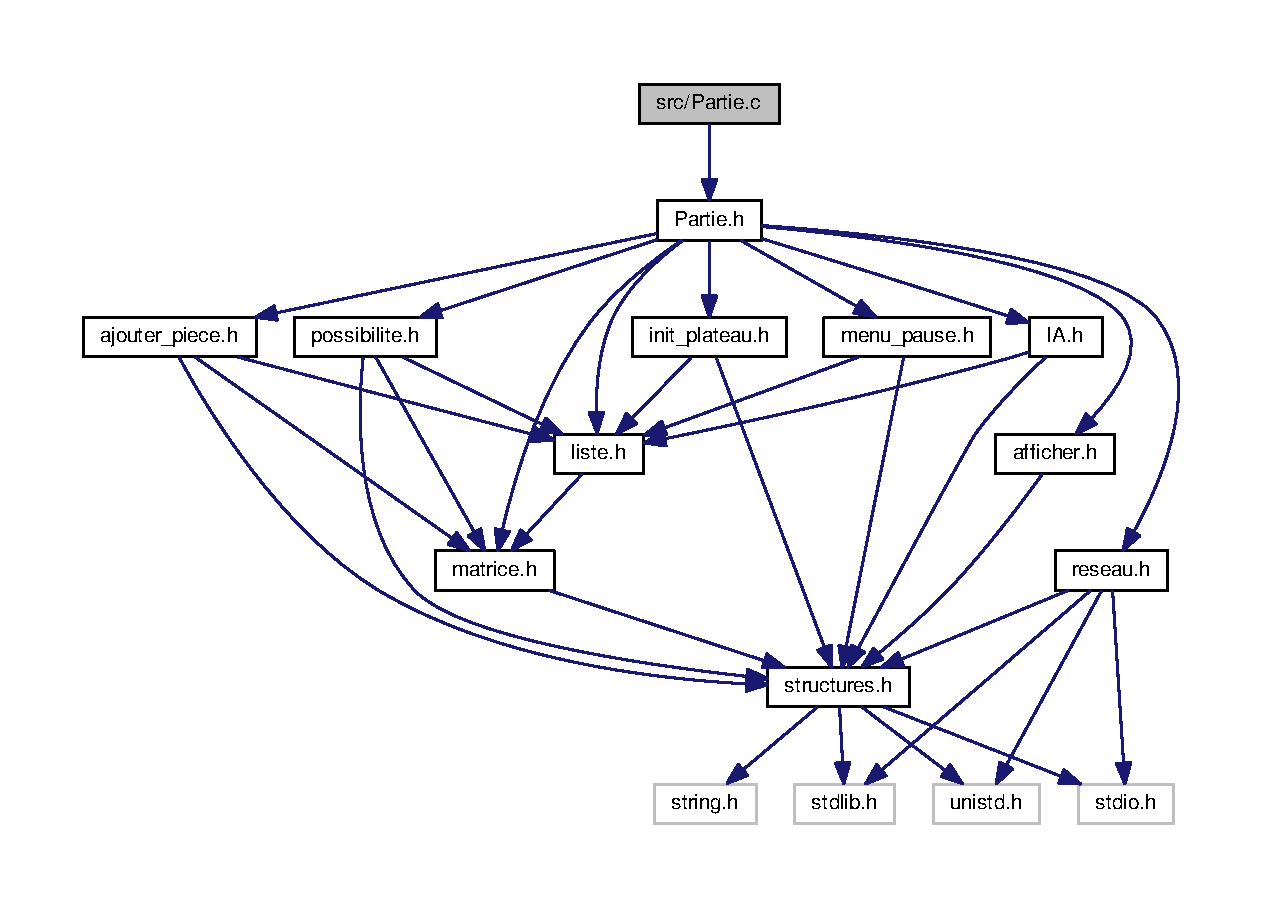
\includegraphics[width=350pt]{Partie_8c__incl}
\end{center}
\end{figure}
\subsection*{Fonctions}
\begin{DoxyCompactItemize}
\item 
void \hyperlink{Partie_8c_a847b594eae4ec1cdf46566486092b06f}{afficher\+\_\+piece\+\_\+dispo} (int nb\+\_\+piece, \hyperlink{structt__liste}{t\+\_\+liste} $\ast$liste)
\begin{DoxyCompactList}\small\item\em Affiche tous les numero des pieces restantes. \end{DoxyCompactList}\item 
int {\bfseries piece\+\_\+dispo} (int num\+\_\+piece\+\_\+choisi, \hyperlink{structt__liste}{t\+\_\+liste} $\ast$liste, \hyperlink{structt__matrice}{t\+\_\+matrice} $\ast$piece)\hypertarget{Partie_8c_a62f643e238582f1badb8b9c46d8ac5bc}{}\label{Partie_8c_a62f643e238582f1badb8b9c46d8ac5bc}

\item 
void {\bfseries calcule\+\_\+score} (int nbj\+\_\+max, int $\ast$score, int joueur, \hyperlink{structt__liste}{t\+\_\+liste} $\ast$liste)\hypertarget{Partie_8c_a55a1332b7c8b99d7450c025a052c98c0}{}\label{Partie_8c_a55a1332b7c8b99d7450c025a052c98c0}

\item 
int {\bfseries jeux} (int nbj, int nbj\+\_\+max, int nb\+\_\+tour\+\_\+joueur, int $\ast$score, int $\ast$joueur\+\_\+en\+\_\+jeux, int taille\+\_\+plateau, \hyperlink{structt__case}{t\+\_\+case}($\ast$plateau)\mbox{[}taille\+\_\+plateau\mbox{]}, \hyperlink{structt__liste}{t\+\_\+liste} $\ast$liste\+\_\+piece, int partie)\hypertarget{Partie_8c_a2cdf8c55e08f9a5b660c54bf6e038f91}{}\label{Partie_8c_a2cdf8c55e08f9a5b660c54bf6e038f91}

\end{DoxyCompactItemize}


\subsection{Description détaillée}
Ensemble de fonctions qui font tourner une partie de jeu. Fichier principal. 

\begin{DoxyAuthor}{Auteur}
Friant Marilou Tourpe Florian Semamra Kevin Amillard Joris 
\end{DoxyAuthor}
\begin{DoxyVersion}{Version}
1 
\end{DoxyVersion}


\subsection{Documentation des fonctions}
\index{Partie.\+c@{Partie.\+c}!afficher\+\_\+piece\+\_\+dispo@{afficher\+\_\+piece\+\_\+dispo}}
\index{afficher\+\_\+piece\+\_\+dispo@{afficher\+\_\+piece\+\_\+dispo}!Partie.\+c@{Partie.\+c}}
\subsubsection[{\texorpdfstring{afficher\+\_\+piece\+\_\+dispo(int nb\+\_\+piece, t\+\_\+liste $\ast$liste)}{afficher_piece_dispo(int nb_piece, t_liste *liste)}}]{\setlength{\rightskip}{0pt plus 5cm}void afficher\+\_\+piece\+\_\+dispo (
\begin{DoxyParamCaption}
\item[{int}]{nb\+\_\+piece, }
\item[{{\bf t\+\_\+liste} $\ast$}]{liste}
\end{DoxyParamCaption}
)}\hypertarget{Partie_8c_a847b594eae4ec1cdf46566486092b06f}{}\label{Partie_8c_a847b594eae4ec1cdf46566486092b06f}


Affiche tous les numero des pieces restantes. 


\begin{DoxyParams}{Paramètres}
{\em nb\+\_\+piece} & num�ro de la pi�ce recerch�e \\
\hline
{\em liste} & Pointeur sur une liste de pi�ces \\
\hline
\end{DoxyParams}

\hypertarget{possibilite_8c}{}\section{Référence du fichier /info/etu/l2info/l2info031/\+Projet\+\_\+blokus-\/\+Version\+\_\+\+Terminale/src/possibilite.c}
\label{possibilite_8c}\index{/info/etu/l2info/l2info031/\+Projet\+\_\+blokus-\/\+Version\+\_\+\+Terminale/src/possibilite.\+c@{/info/etu/l2info/l2info031/\+Projet\+\_\+blokus-\/\+Version\+\_\+\+Terminale/src/possibilite.\+c}}


Ensemble de fonctions relatives aux possibilitees du positionnement d\textquotesingle{}une ou de plusieurs piece avec un plateau donne.  


{\ttfamily \#include \char`\"{}possibilite.\+h\char`\"{}}\\*
{\ttfamily \#include \char`\"{}init\+\_\+plateau.\+h\char`\"{}}\\*
{\ttfamily \#include \char`\"{}ajouter\+\_\+piece.\+h\char`\"{}}\\*
Graphe des dépendances par inclusion de possibilite.\+c\+:\nopagebreak
\begin{figure}[H]
\begin{center}
\leavevmode
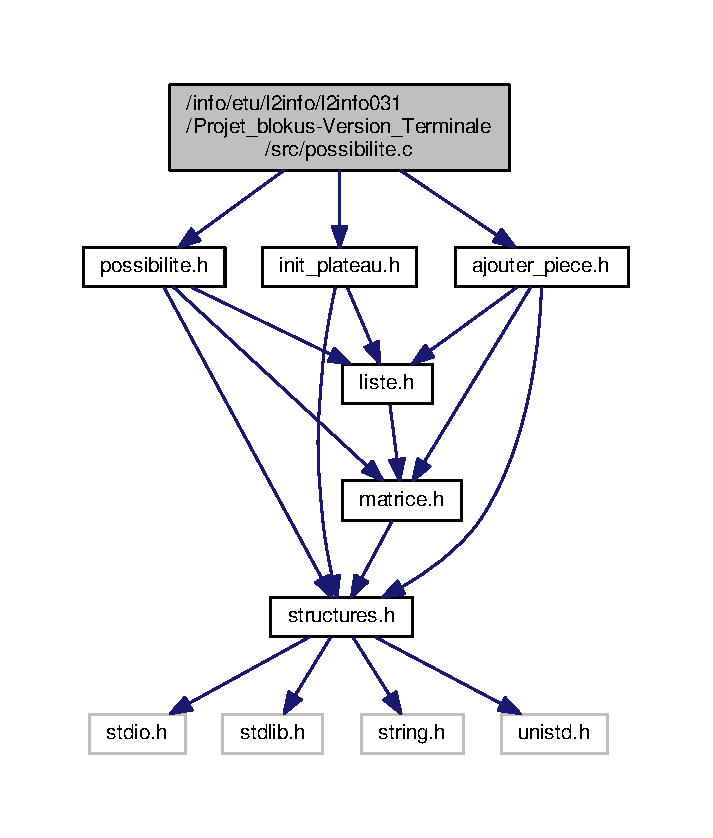
\includegraphics[width=342pt]{possibilite_8c__incl}
\end{center}
\end{figure}
\subsection*{Fonctions}
\begin{DoxyCompactItemize}
\item 
int {\bfseries verif\+\_\+posibiliter} (int nb\+\_\+tour, \hyperlink{structt__coordonnee}{t\+\_\+coordonnee} $\ast$$\ast$tab\+\_\+dispo, int joueur, int $\ast$nb\+\_\+dispo, \hyperlink{structt__liste}{t\+\_\+liste} $\ast$liste, int taille\+\_\+plateau, \hyperlink{structt__case}{t\+\_\+case}($\ast$plateau)\mbox{[}taille\+\_\+plateau\mbox{]})\hypertarget{possibilite_8c_ab35679c28a8eac54813f8e47e374447c}{}\label{possibilite_8c_ab35679c28a8eac54813f8e47e374447c}

\item 
int {\bfseries possible\+\_\+de\+\_\+jouer} (int taille\+\_\+plateau, \hyperlink{structt__case}{t\+\_\+case}($\ast$plateau)\mbox{[}taille\+\_\+plateau\mbox{]}, int joueur, int nb\+\_\+tour, \hyperlink{structt__coordonnee}{t\+\_\+coordonnee} $\ast$$\ast$tab\+\_\+dispo, int $\ast$nb\+\_\+dispo, \hyperlink{structt__liste}{t\+\_\+liste} $\ast$liste)\hypertarget{possibilite_8c_afef4355ae5dbf5cd66db9c1f525156e3}{}\label{possibilite_8c_afef4355ae5dbf5cd66db9c1f525156e3}

\end{DoxyCompactItemize}


\subsection{Description détaillée}
Ensemble de fonctions relatives aux possibilitees du positionnement d\textquotesingle{}une ou de plusieurs piece avec un plateau donne. 

\begin{DoxyAuthor}{Auteur}
Friant Marilou Tourpe Florian Semamra Kevin Amillard Joris 
\end{DoxyAuthor}
\begin{DoxyVersion}{Version}
1 
\end{DoxyVersion}

\hypertarget{reseau_8c}{}\section{reseau.\+c File Reference}
\label{reseau_8c}\index{reseau.\+c@{reseau.\+c}}


Module qui permet une connexion T\+CP entre plusieurs ordinateurs.  


{\ttfamily \#include \char`\"{}reseau.\+h\char`\"{}}\newline
\subsection*{Functions}
\begin{DoxyCompactItemize}
\item 
void \mbox{\hyperlink{reseau_8c_add6e60e086591b7a1bd273bde5add9e7}{init\+\_\+serveur}} (int $\ast$socket\+\_\+serveur, struct sockaddr\+\_\+in $\ast$adresse\+\_\+serveur)
\begin{DoxyCompactList}\small\item\em Instaure un socket serveur sur l\textquotesingle{}ordinateur. \end{DoxyCompactList}\item 
void \mbox{\hyperlink{reseau_8c_a15751481a827478277413657b08134c3}{ajout\+\_\+clients}} (int $\ast$socket\+\_\+serveur, int socket\+\_\+client \mbox{[}$\,$\mbox{]}, int nbj\+\_\+max)
\begin{DoxyCompactList}\small\item\em Ajoute des clients sur des sockets clients. \end{DoxyCompactList}\item 
int \mbox{\hyperlink{reseau_8c_ae9e47c397f69d8c57e3fe7fb4b84d152}{connexion\+\_\+serveur}} (int $\ast$socket\+\_\+client, struct sockaddr\+\_\+in $\ast$server\+\_\+address)
\begin{DoxyCompactList}\small\item\em Foctio qui permet de se conecter à un serveur. \end{DoxyCompactList}\item 
void \mbox{\hyperlink{reseau_8c_a41db51cf896f92d120012c45b9e62345}{envoyer\+\_\+plateau\+\_\+clients}} (int socket\+\_\+client \mbox{[}$\,$\mbox{]}, int taille\+\_\+plateau, \mbox{\hyperlink{structt__case}{t\+\_\+case}}($\ast$plateau) \mbox{[}taille\+\_\+plateau\mbox{]}, int nbj\+\_\+max)
\begin{DoxyCompactList}\small\item\em Envoie le plateau de jeu à tous les clients. \end{DoxyCompactList}\item 
void \mbox{\hyperlink{reseau_8c_a8ad56034f582019021feed3dee3128bd}{envoyer\+\_\+plateau}} (int socket\+\_\+client, int taille\+\_\+plateau, \mbox{\hyperlink{structt__case}{t\+\_\+case}}($\ast$plateau) \mbox{[}taille\+\_\+plateau\mbox{]})
\begin{DoxyCompactList}\small\item\em Envoie le plateau de jeu. \end{DoxyCompactList}\item 
void \mbox{\hyperlink{reseau_8c_aea0fee6be243dadc9e9a35d633143994}{envoyer\+\_\+numero}} (int socket\+\_\+client, int numero)
\begin{DoxyCompactList}\small\item\em Envoie un numéro qui est attribué au joueur. \end{DoxyCompactList}\item 
void \mbox{\hyperlink{reseau_8c_a18c2033e4cad10017063c9dc85ac8028}{nv\+\_\+plateau}} (int socket\+\_\+client, int taille\+\_\+plateau, \mbox{\hyperlink{structt__case}{t\+\_\+case}}($\ast$plateau) \mbox{[}taille\+\_\+plateau\mbox{]})
\begin{DoxyCompactList}\small\item\em Reçoit le nouvel état du plateau de jeu. \end{DoxyCompactList}\end{DoxyCompactItemize}


\subsection{Detailed Description}
Module qui permet une connexion T\+CP entre plusieurs ordinateurs. 

\begin{DoxyAuthor}{Author}
Friant Marilou Tourpe Florian Semamra Kevin Amillard Joris 
\end{DoxyAuthor}
\begin{DoxyVersion}{Version}
1 
\end{DoxyVersion}


\subsection{Function Documentation}
\mbox{\Hypertarget{reseau_8c_a15751481a827478277413657b08134c3}\label{reseau_8c_a15751481a827478277413657b08134c3}} 
\index{reseau.\+c@{reseau.\+c}!ajout\+\_\+clients@{ajout\+\_\+clients}}
\index{ajout\+\_\+clients@{ajout\+\_\+clients}!reseau.\+c@{reseau.\+c}}
\subsubsection{\texorpdfstring{ajout\+\_\+clients()}{ajout\_clients()}}
{\footnotesize\ttfamily void ajout\+\_\+clients (\begin{DoxyParamCaption}\item[{int $\ast$}]{socket\+\_\+serveur,  }\item[{int}]{socket\+\_\+client\mbox{[}$\,$\mbox{]},  }\item[{int}]{nbj\+\_\+max }\end{DoxyParamCaption})}



Ajoute des clients sur des sockets clients. 


\begin{DoxyParams}{Parameters}
{\em $\ast$socket\+\_\+serveur} & le socket serveur \\
\hline
{\em socket\+\_\+client\mbox{[}$\,$\mbox{]}} & Les sockets clients à lier au serveur \\
\hline
{\em nbj\+\_\+max} & Le nombre de clients à lier \\
\hline
\end{DoxyParams}
\mbox{\Hypertarget{reseau_8c_ae9e47c397f69d8c57e3fe7fb4b84d152}\label{reseau_8c_ae9e47c397f69d8c57e3fe7fb4b84d152}} 
\index{reseau.\+c@{reseau.\+c}!connexion\+\_\+serveur@{connexion\+\_\+serveur}}
\index{connexion\+\_\+serveur@{connexion\+\_\+serveur}!reseau.\+c@{reseau.\+c}}
\subsubsection{\texorpdfstring{connexion\+\_\+serveur()}{connexion\_serveur()}}
{\footnotesize\ttfamily int connexion\+\_\+serveur (\begin{DoxyParamCaption}\item[{int $\ast$}]{socket\+\_\+client,  }\item[{struct sockaddr\+\_\+in $\ast$}]{server\+\_\+address }\end{DoxyParamCaption})}



Foctio qui permet de se conecter à un serveur. 


\begin{DoxyParams}{Parameters}
{\em $\ast$socket\+\_\+client} & le socket du client \\
\hline
{\em $\ast$server\+\_\+address} & Les informations du serveur à indiquer \\
\hline
\end{DoxyParams}
\mbox{\Hypertarget{reseau_8c_aea0fee6be243dadc9e9a35d633143994}\label{reseau_8c_aea0fee6be243dadc9e9a35d633143994}} 
\index{reseau.\+c@{reseau.\+c}!envoyer\+\_\+numero@{envoyer\+\_\+numero}}
\index{envoyer\+\_\+numero@{envoyer\+\_\+numero}!reseau.\+c@{reseau.\+c}}
\subsubsection{\texorpdfstring{envoyer\+\_\+numero()}{envoyer\_numero()}}
{\footnotesize\ttfamily void envoyer\+\_\+numero (\begin{DoxyParamCaption}\item[{int}]{socket\+\_\+client,  }\item[{int}]{numero }\end{DoxyParamCaption})}



Envoie un numéro qui est attribué au joueur. 


\begin{DoxyParams}{Parameters}
{\em socket\+\_\+client} & le socket du client \\
\hline
{\em numero} & le numéro attribué au joueur \\
\hline
\end{DoxyParams}
\mbox{\Hypertarget{reseau_8c_a8ad56034f582019021feed3dee3128bd}\label{reseau_8c_a8ad56034f582019021feed3dee3128bd}} 
\index{reseau.\+c@{reseau.\+c}!envoyer\+\_\+plateau@{envoyer\+\_\+plateau}}
\index{envoyer\+\_\+plateau@{envoyer\+\_\+plateau}!reseau.\+c@{reseau.\+c}}
\subsubsection{\texorpdfstring{envoyer\+\_\+plateau()}{envoyer\_plateau()}}
{\footnotesize\ttfamily void envoyer\+\_\+plateau (\begin{DoxyParamCaption}\item[{int}]{socket\+\_\+client,  }\item[{int}]{taille\+\_\+plateau,  }\item[{\mbox{\hyperlink{structt__case}{t\+\_\+case}}($\ast$)}]{plateau\mbox{[}taille\+\_\+plateau\mbox{]} }\end{DoxyParamCaption})}



Envoie le plateau de jeu. 


\begin{DoxyParams}{Parameters}
{\em socket\+\_\+client} & le socket du client \\
\hline
{\em taille\+\_\+plateau} & La taille du plateau de jeu \\
\hline
{\em ($\ast$plateau)\mbox{[}taille\+\_\+plateau\mbox{]}} & Le plateau de jeu \\
\hline
\end{DoxyParams}
\mbox{\Hypertarget{reseau_8c_a41db51cf896f92d120012c45b9e62345}\label{reseau_8c_a41db51cf896f92d120012c45b9e62345}} 
\index{reseau.\+c@{reseau.\+c}!envoyer\+\_\+plateau\+\_\+clients@{envoyer\+\_\+plateau\+\_\+clients}}
\index{envoyer\+\_\+plateau\+\_\+clients@{envoyer\+\_\+plateau\+\_\+clients}!reseau.\+c@{reseau.\+c}}
\subsubsection{\texorpdfstring{envoyer\+\_\+plateau\+\_\+clients()}{envoyer\_plateau\_clients()}}
{\footnotesize\ttfamily void envoyer\+\_\+plateau\+\_\+clients (\begin{DoxyParamCaption}\item[{int}]{socket\+\_\+client\mbox{[}$\,$\mbox{]},  }\item[{int}]{taille\+\_\+plateau,  }\item[{\mbox{\hyperlink{structt__case}{t\+\_\+case}}($\ast$)}]{plateau\mbox{[}taille\+\_\+plateau\mbox{]},  }\item[{int}]{nbj\+\_\+max }\end{DoxyParamCaption})}



Envoie le plateau de jeu à tous les clients. 


\begin{DoxyParams}{Parameters}
{\em socket\+\_\+client\mbox{[}$\,$\mbox{]}} & les sockets des clients \\
\hline
{\em $\ast$taille\+\_\+plateau} & La taille du plateau de jeu \\
\hline
{\em ($\ast$plateau)\mbox{[}taille\+\_\+plateau\mbox{]}} & Le plateau de jeu \\
\hline
{\em nbj\+\_\+max} & Le nombre de joueurs \\
\hline
\end{DoxyParams}
\mbox{\Hypertarget{reseau_8c_add6e60e086591b7a1bd273bde5add9e7}\label{reseau_8c_add6e60e086591b7a1bd273bde5add9e7}} 
\index{reseau.\+c@{reseau.\+c}!init\+\_\+serveur@{init\+\_\+serveur}}
\index{init\+\_\+serveur@{init\+\_\+serveur}!reseau.\+c@{reseau.\+c}}
\subsubsection{\texorpdfstring{init\+\_\+serveur()}{init\_serveur()}}
{\footnotesize\ttfamily void init\+\_\+serveur (\begin{DoxyParamCaption}\item[{int $\ast$}]{socket\+\_\+serveur,  }\item[{struct sockaddr\+\_\+in $\ast$}]{adresse\+\_\+serveur }\end{DoxyParamCaption})}



Instaure un socket serveur sur l\textquotesingle{}ordinateur. 


\begin{DoxyParams}{Parameters}
{\em $\ast$socket\+\_\+serveur} & le socket serveur à initialiser \\
\hline
{\em $\ast$adresse\+\_\+serveur} & informations sur l\textquotesingle{}adresse du pc \\
\hline
\end{DoxyParams}
\mbox{\Hypertarget{reseau_8c_a18c2033e4cad10017063c9dc85ac8028}\label{reseau_8c_a18c2033e4cad10017063c9dc85ac8028}} 
\index{reseau.\+c@{reseau.\+c}!nv\+\_\+plateau@{nv\+\_\+plateau}}
\index{nv\+\_\+plateau@{nv\+\_\+plateau}!reseau.\+c@{reseau.\+c}}
\subsubsection{\texorpdfstring{nv\+\_\+plateau()}{nv\_plateau()}}
{\footnotesize\ttfamily void nv\+\_\+plateau (\begin{DoxyParamCaption}\item[{int}]{socket\+\_\+client,  }\item[{int}]{taille\+\_\+plateau,  }\item[{\mbox{\hyperlink{structt__case}{t\+\_\+case}}($\ast$)}]{plateau\mbox{[}taille\+\_\+plateau\mbox{]} }\end{DoxyParamCaption})}



Reçoit le nouvel état du plateau de jeu. 


\begin{DoxyParams}{Parameters}
{\em taille\+\_\+plateau} & La taille du plateau de jeu \\
\hline
{\em ($\ast$plateau)\mbox{[}taille\+\_\+plateau\mbox{]}} & Le plateau de jeu \\
\hline
\end{DoxyParams}

\hypertarget{structures_8h}{}\section{Référence du fichier /info/etu/l2info/l2info031/\+Projet\+\_\+blokus-\/\+Version\+\_\+\+Terminale/src/structures.h}
\label{structures_8h}\index{/info/etu/l2info/l2info031/\+Projet\+\_\+blokus-\/\+Version\+\_\+\+Terminale/src/structures.\+h@{/info/etu/l2info/l2info031/\+Projet\+\_\+blokus-\/\+Version\+\_\+\+Terminale/src/structures.\+h}}


Contient les structures communes du programme.  


{\ttfamily \#include $<$stdio.\+h$>$}\\*
{\ttfamily \#include $<$stdlib.\+h$>$}\\*
{\ttfamily \#include $<$string.\+h$>$}\\*
{\ttfamily \#include $<$unistd.\+h$>$}\\*
Graphe des dépendances par inclusion de structures.\+h\+:\nopagebreak
\begin{figure}[H]
\begin{center}
\leavevmode
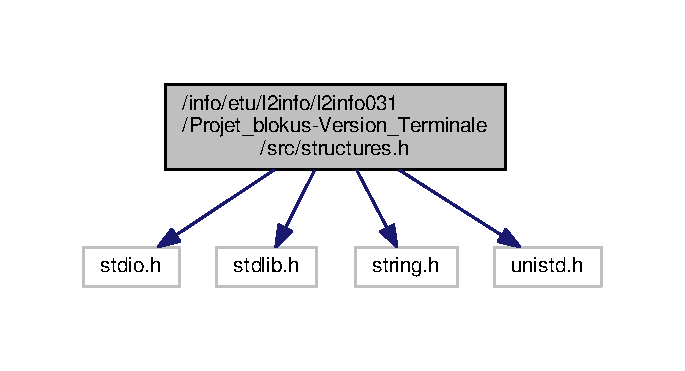
\includegraphics[width=329pt]{structures_8h__incl}
\end{center}
\end{figure}
Ce graphe montre quels fichiers incluent directement ou indirectement ce fichier \+:
\nopagebreak
\begin{figure}[H]
\begin{center}
\leavevmode
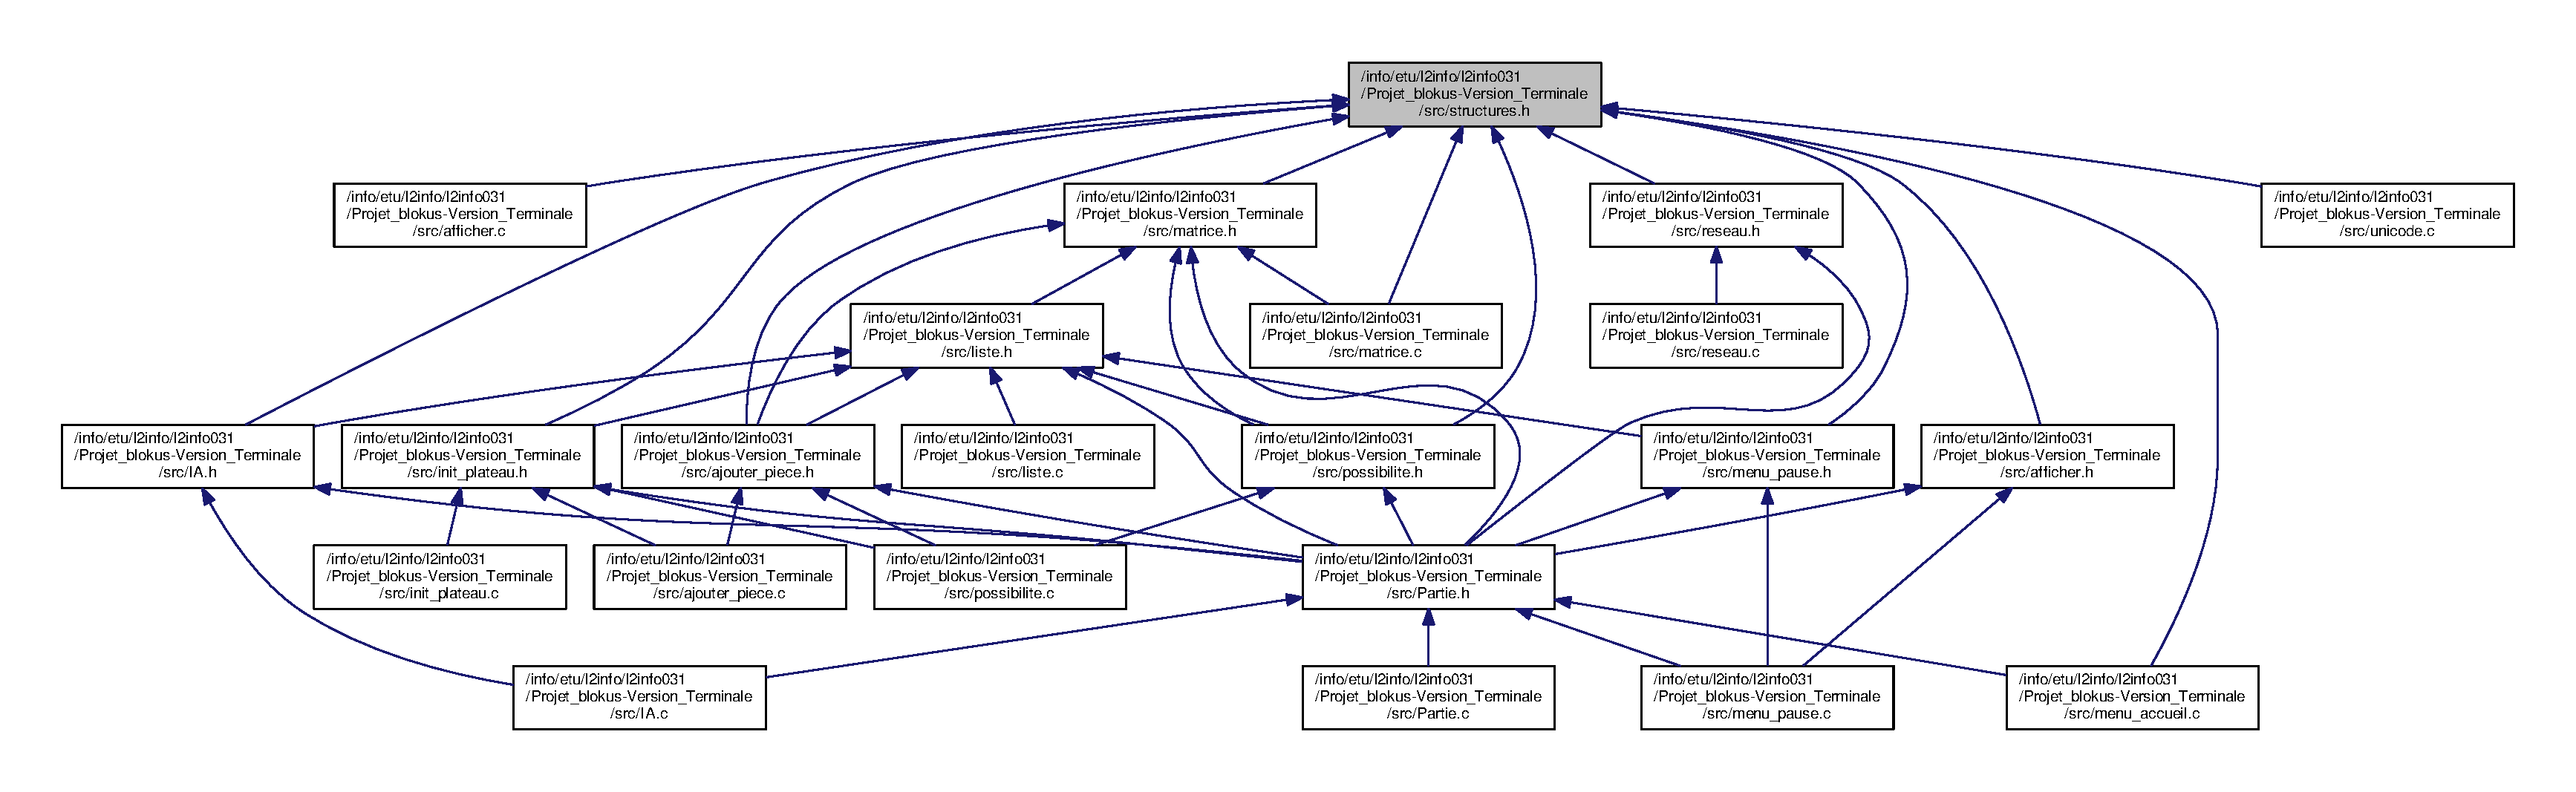
\includegraphics[width=350pt]{structures_8h__dep__incl}
\end{center}
\end{figure}
\subsection*{Classes}
\begin{DoxyCompactItemize}
\item 
struct \hyperlink{structt__case}{t\+\_\+case}
\begin{DoxyCompactList}\small\item\em Définition d\textquotesingle{}une case pour un plateau de Blokus. \end{DoxyCompactList}\item 
struct \hyperlink{structt__coordonnee}{t\+\_\+coordonnee}
\begin{DoxyCompactList}\small\item\em Contient des coordonnées pour une matrice à deux dimensions. \end{DoxyCompactList}\end{DoxyCompactItemize}
\subsection*{Macros}
\begin{DoxyCompactItemize}
\item 
\#define {\bfseries T\+A\+I\+L\+L\+E\+\_\+\+M\+AX}~21\hypertarget{structures_8h_ae6ad0540d5109a0200f0dde5dc5b4bf6}{}\label{structures_8h_ae6ad0540d5109a0200f0dde5dc5b4bf6}

\item 
\#define {\bfseries T\+A\+I\+L\+L\+E\+\_\+\+M\+A\+T\+R\+I\+C\+E\+\_\+\+P\+I\+E\+CE}~5\hypertarget{structures_8h_a93a84f484a79b425fbe94baedfbbac48}{}\label{structures_8h_a93a84f484a79b425fbe94baedfbbac48}

\end{DoxyCompactItemize}
\subsection*{Énumérations}
\begin{DoxyCompactItemize}
\item 
enum \hyperlink{structures_8h_aa9f0f93fc533400ebe242cbb9986ef07}{t\+\_\+couleur} \{ \\*
\hyperlink{structures_8h_aa9f0f93fc533400ebe242cbb9986ef07ac2a84c546ae51a97ad3a356f791e371e}{libre} = 4, 
{\bfseries rouge} = 0, 
{\bfseries bleu} = 1, 
{\bfseries vert} = 2, 
\\*
{\bfseries jaune} = 3
 \}\begin{DoxyCompactList}\small\item\em Définition de couleurs en fonction d\textquotesingle{}un entier. \end{DoxyCompactList}
\end{DoxyCompactItemize}


\subsection{Description détaillée}
Contient les structures communes du programme. 

\begin{DoxyVersion}{Version}
1.\+0 
\end{DoxyVersion}
\begin{DoxyDate}{Date}
mars 2018 
\end{DoxyDate}


\subsection{Documentation du type de l\textquotesingle{}énumération}
\index{structures.\+h@{structures.\+h}!t\+\_\+couleur@{t\+\_\+couleur}}
\index{t\+\_\+couleur@{t\+\_\+couleur}!structures.\+h@{structures.\+h}}
\subsubsection[{\texorpdfstring{t\+\_\+couleur}{t_couleur}}]{\setlength{\rightskip}{0pt plus 5cm}enum {\bf t\+\_\+couleur}}\hypertarget{structures_8h_aa9f0f93fc533400ebe242cbb9986ef07}{}\label{structures_8h_aa9f0f93fc533400ebe242cbb9986ef07}


Définition de couleurs en fonction d\textquotesingle{}un entier. 

L\textquotesingle{}énumération contient les quatre couleurs utilisées pour le Blokus ainsi qu\textquotesingle{}une valeur utilisée si aucune couleur n\textquotesingle{}est présente \begin{Desc}
\item[Valeurs énumérées]\par
\begin{description}
\index{libre@{libre}!structures.\+h@{structures.\+h}}\index{structures.\+h@{structures.\+h}!libre@{libre}}\item[{\em 
libre\hypertarget{structures_8h_aa9f0f93fc533400ebe242cbb9986ef07ac2a84c546ae51a97ad3a356f791e371e}{}\label{structures_8h_aa9f0f93fc533400ebe242cbb9986ef07ac2a84c546ae51a97ad3a356f791e371e}
}]Sans couleur \end{description}
\end{Desc}

\hypertarget{unicode_8c}{}\section{Référence du fichier src/unicode.c}
\label{unicode_8c}\index{src/unicode.\+c@{src/unicode.\+c}}


Fonctions d\textquotesingle{}affichage des cases du plateau avec des caractères unicode.  


{\ttfamily \#include $<$stdlib.\+h$>$}\\*
{\ttfamily \#include $<$stdio.\+h$>$}\\*
{\ttfamily \#include \char`\"{}unicode.\+h\char`\"{}}\\*
{\ttfamily \#include \char`\"{}couleurs.\+h\char`\"{}}\\*
{\ttfamily \#include \char`\"{}structures.\+h\char`\"{}}\\*
Graphe des dépendances par inclusion de unicode.\+c\+:
\nopagebreak
\begin{figure}[H]
\begin{center}
\leavevmode
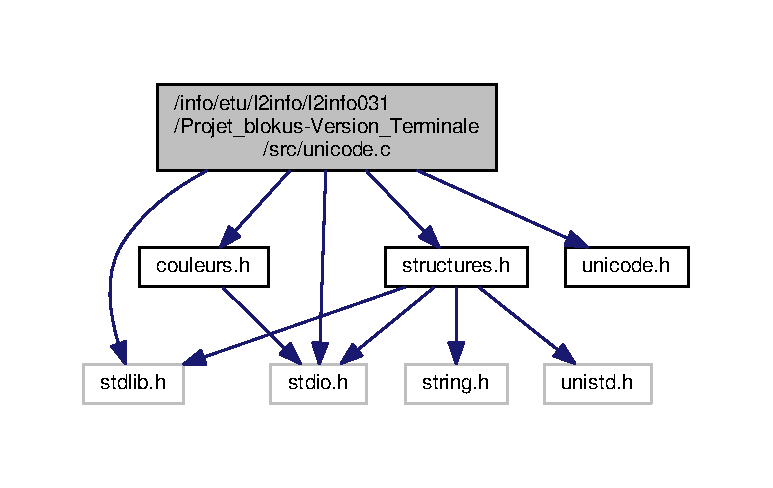
\includegraphics[width=350pt]{unicode_8c__incl}
\end{center}
\end{figure}
\subsection*{Fonctions}
\begin{DoxyCompactItemize}
\item 
void \hyperlink{unicode_8c_a61ef8e58ec8fff2bd2273058a38b7689}{aff\+\_\+case\+\_\+haut} (int x, int y, int couleur, int nb\+\_\+joueurs)
\begin{DoxyCompactList}\small\item\em Affiche le haut d\textquotesingle{}une case du plateau. \end{DoxyCompactList}\item 
void \hyperlink{unicode_8c_a2756c6713422f9de9a781715d15da33b}{aff\+\_\+case\+\_\+bas} (int x, int y, int couleur, int nb\+\_\+joueurs)
\begin{DoxyCompactList}\small\item\em Affiche le bas d\textquotesingle{}une case du plateau. \end{DoxyCompactList}\end{DoxyCompactItemize}


\subsection{Description détaillée}
Fonctions d\textquotesingle{}affichage des cases du plateau avec des caractères unicode. 

Contient deux fonctions pour l\textquotesingle{}affichage du haut d\textquotesingle{}une case et du bas d\textquotesingle{}une case en caractère unicode et avec gestion de couleur. Les caractères unicodes sont directement rentrés dans le code car sinon les lignes du plateau ne s\textquotesingle{}alignent pas correctement. \begin{DoxyAuthor}{Auteur}
Kevin Semamra 
\end{DoxyAuthor}
\begin{DoxyVersion}{Version}
1.\+0 
\end{DoxyVersion}
\begin{DoxyDate}{Date}
mars 2018 
\end{DoxyDate}


\subsection{Documentation des fonctions}
\index{unicode.\+c@{unicode.\+c}!aff\+\_\+case\+\_\+bas@{aff\+\_\+case\+\_\+bas}}
\index{aff\+\_\+case\+\_\+bas@{aff\+\_\+case\+\_\+bas}!unicode.\+c@{unicode.\+c}}
\subsubsection[{\texorpdfstring{aff\+\_\+case\+\_\+bas(int x, int y, int couleur, int nb\+\_\+joueurs)}{aff_case_bas(int x, int y, int couleur, int nb_joueurs)}}]{\setlength{\rightskip}{0pt plus 5cm}void aff\+\_\+case\+\_\+bas (
\begin{DoxyParamCaption}
\item[{int}]{x, }
\item[{int}]{y, }
\item[{int}]{couleur, }
\item[{int}]{nb\+\_\+joueurs}
\end{DoxyParamCaption}
)}\hypertarget{unicode_8c_a2756c6713422f9de9a781715d15da33b}{}\label{unicode_8c_a2756c6713422f9de9a781715d15da33b}


Affiche le bas d\textquotesingle{}une case du plateau. 

Affiche les bordures de la partie basse de la case, ainsi que la couleur correspondant à une pièce ou une possibilité de placement pour le joueur courant. 
\begin{DoxyParams}{Paramètres}
{\em x} & x représente un numéro de colonne. \\
\hline
{\em y} & y représente un numéro de ligne. \\
\hline
{\em nb\+\_\+joueurs} & nb\+\_\+joueurs est utilisé pour déterminé la longueur du plateau. \\
\hline
\end{DoxyParams}
\index{unicode.\+c@{unicode.\+c}!aff\+\_\+case\+\_\+haut@{aff\+\_\+case\+\_\+haut}}
\index{aff\+\_\+case\+\_\+haut@{aff\+\_\+case\+\_\+haut}!unicode.\+c@{unicode.\+c}}
\subsubsection[{\texorpdfstring{aff\+\_\+case\+\_\+haut(int x, int y, int couleur, int nb\+\_\+joueurs)}{aff_case_haut(int x, int y, int couleur, int nb_joueurs)}}]{\setlength{\rightskip}{0pt plus 5cm}void aff\+\_\+case\+\_\+haut (
\begin{DoxyParamCaption}
\item[{int}]{x, }
\item[{int}]{y, }
\item[{int}]{couleur, }
\item[{int}]{nb\+\_\+joueurs}
\end{DoxyParamCaption}
)}\hypertarget{unicode_8c_a61ef8e58ec8fff2bd2273058a38b7689}{}\label{unicode_8c_a61ef8e58ec8fff2bd2273058a38b7689}


Affiche le haut d\textquotesingle{}une case du plateau. 

Affiche les bordures de la partie haute de la case, ainsi que la couleur correspondant à une pièce ou une possibilité de placement pour le joueur courant. 
\begin{DoxyParams}{Paramètres}
{\em x} & x représente un numéro de colonne. \\
\hline
{\em y} & y représente un numéro de ligne. \\
\hline
{\em nb\+\_\+joueurs} & nb\+\_\+joueurs est utilisé pour déterminé la longueur du plateau. \\
\hline
\end{DoxyParams}

%--- End generated contents ---

% Index
\backmatter
\newpage
\phantomsection
\clearemptydoublepage
\addcontentsline{toc}{chapter}{Index}
\printindex

\end{document}
